\documentclass[a4paper, openany]{book}
%\documentclass{tuftebook}
\usepackage{graphicx}
\usepackage[export]{adjustbox}
\usepackage{amsthm}
\usepackage[many]{tcolorbox}
\usepackage[margin=0.75in]{geometry}
\usepackage{amsmath,amssymb,amsfonts}
\usepackage{mathtools}
\usepackage{enumerate}
\usepackage{wrapfig}
\usepackage[makeroom]{cancel}
\usepackage{nameref}
\usepackage{xparse}
\usepackage{tikz}
\usepackage{wrapfig} % <-- important
\usepackage{cancel}
\usepackage[colorlinks = true, linkcolor = black]{hyperref}
\usepackage{multicol}
\usepackage{tikz-cd}

\usetikzlibrary{arrows.meta}
\usetikzlibrary{matrix}

\makeatletter

\makeatletter

\def\renewtheorem#1{%
	\expandafter\let\csname#1\endcsname\relax
	\expandafter\let\csname c@#1\endcsname\relax
	\gdef\renewtheorem@envname{#1}
	\renewtheorem@secpar
}
\def\renewtheorem@secpar{\@ifnextchar[{\renewtheorem@numberedlike}{\renewtheorem@nonumberedlike}}
\def\renewtheorem@numberedlike[#1]#2{\newtheorem{\renewtheorem@envname}[#1]{#2}}
\def\renewtheorem@nonumberedlike#1{
	\def\renewtheorem@caption{#1}
	\edef\renewtheorem@nowithin{\noexpand\newtheorem{\renewtheorem@envname}{\renewtheorem@caption}}
	\renewtheorem@thirdpar
}
\def\renewtheorem@thirdpar{\@ifnextchar[{\renewtheorem@within}{\renewtheorem@nowithin}}
\def\renewtheorem@within[#1]{\renewtheorem@nowithin[#1]}

\makeatother

%sets enumerate to roman numerals
\renewcommand{\labelenumi}{(\roman{enumi})}
\renewcommand{\theenumi}{\roman{enumi}}
\renewcommand{\labelenumii}{(\alph{enumii})}
\renewcommand{\theenumii}{\alph{enumii}}

%%%%%%%%%%%%%%%%%%%%
% New environments %
%%%%%%%%%%%%%%%%%%%%

\makeatother
%\mdfsetup{skipabove=1em,skipbelow=0em}

\tcbuselibrary{skins}

% Color definitions

\definecolor{proofcolor}{RGB}{0,0,0}

% Dark orange and Dark Red rgb
%\definecolor{theorembordercolor}{RGB}{151, 63, 5}
%\definecolor{theorembackgroundcolor}{RGB}{248, 241, 234}
\definecolor{theorembordercolor}{RGB}{255, 165, 0}
\definecolor{theorembackgroundcolor}{RGB}{254, 249, 243}

%\definecolor{examplebordercolor}{RGB}{0, 110, 184}
\definecolor{remarkbackgroundcolor}{RGB}{240, 244, 250}

\definecolor{examplebordercolor}{RGB}{199, 0, 57}
\definecolor{examplebackgroundcolor}{RGB}{248, 241, 234}

\definecolor{remarkbordercolor}{RGB}{0, 110, 184}

\definecolor{definitionbordercolor}{RGB}{0, 150, 85}
\definecolor{definitionbackgroundcolor}{RGB}{239, 247, 243}

\definecolor{propertybordercolor}{RGB}{128, 0, 128}
\definecolor{propertybackgroundcolor}{RGB}{255, 240, 255}

\definecolor{formulabordercolor}{RGB}{0, 0, 0}
\definecolor{formulabackgroundcolor}{RGB}{230, 229, 245}

\newtheoremstyle{theorem}
{0pt}{0pt}{\normalfont}{0pt}
{}{\;}{0.25em}
{{\sffamily\bfseries\color{theorembordercolor}\thmname{#1}~\thmnumber{\textup{#2}}.}
	\thmnote{\normalfont\color{black}~(#3)}}

\newtheoremstyle{definition}
{0pt}{0pt}{\normalfont}{0pt}
{}{\;}{0.25em}
{{\sffamily\bfseries\color{definitionbordercolor}\thmname{#1}~\thmnumber{\textup{#2}}.}
	\thmnote{\normalfont\color{black}~(#3)}}

\newtheoremstyle{notation}
{0pt}{0pt}{\normalfont}{0pt}
{}{\;}{0.25em}
{{\sffamily\bfseries\color{definitionbordercolor}\thmname{#1}~\thmnumber{\textup{#2}}.}
	\thmnote{\normalfont\color{black}~(#3)}}

\newtheoremstyle{example}
{0pt}{0pt}{\normalfont}{0pt}
{}{\;}{0.25em}
{{\sffamily\bfseries\color{examplebordercolor}\thmname{#1}~\thmnumber{\textup{#2}}.}
	\thmnote{\normalfont\color{black}~(#3)}}
	
\newtheoremstyle{remark}
{0pt}{0pt}{\normalfont}{0pt}
{}{\;}{0.25em}
{{\sffamily\bfseries\color{remarkbordercolor}\thmname{#1}~\thmnumber{\textup{#2}}.}
	\thmnote{\normalfont\color{black}~(#3)}}	

\newtheoremstyle{property}
{0pt}{0pt}{\normalfont}{0pt}
{}{\;}{0.25em}
{{\sffamily\bfseries\color{propertybordercolor}\thmname{#1}~\thmnumber{\textup{#2}}.}
	\thmnote{\normalfont\color{black}~(#3)}}

\newtheoremstyle{formula}
{0pt}{0pt}{\normalfont}{0pt}
{}{\;}{0.25em}
{{\sffamily\bfseries\color{formulabordercolor}\thmname{#1}~\thmnumber{\textup{#2}}.}
	\thmnote{\normalfont\color{black}~(#3)}}

%%%%%%%%%%%%%%%%%%%%%%%%
% Theorem Environments %
%%%%%%%%%%%%%%%%%%%%%%%%

\theoremstyle{theorem}

\newtheorem{theorem}{Theorem}
\newtheorem{contrapositive}{Contrapositive}
\numberwithin{theorem}{section}
\numberwithin{contrapositive}{section}
\newtheorem{postulate}{Postulate}
%\newtheorem{conjecture}{Conjecture}
%\newtheorem{corollary}{Corollary}
%\newtheorem{lemma}{Lemma}
\newtheorem{conclusion}{Conclusion}

\tcolorboxenvironment{theorem}{
	enhanced jigsaw, pad at break*=1mm, breakable,
	left=4mm, right=4mm, top=1mm, bottom=1mm,
	colback=theorembackgroundcolor, boxrule=0pt, frame hidden,
	borderline west={0.5mm}{0mm}{theorembordercolor}, arc=.5mm
}
\tcolorboxenvironment{contrapositive}{
	enhanced jigsaw, pad at break*=1mm, breakable,
	left=4mm, right=4mm, top=1mm, bottom=1mm,
	colback=theorembackgroundcolor, boxrule=0pt, frame hidden,
	borderline west={0.5mm}{0mm}{theorembordercolor}, arc=.5mm
}
\tcolorboxenvironment{postulate}{
	enhanced jigsaw, pad at break*=1mm, breakable,
	left=4mm, right=4mm, top=1mm, bottom=1mm,
	colback=theorembackgroundcolor, boxrule=0pt, frame hidden,
	borderline west={0.5mm}{0mm}{theorembordercolor}, arc=.5mm
}

%\tcolorboxenvironment{corollary}{
%	enhanced jigsaw, pad at break*=1mm, breakable,
%	left=4mm, right=4mm, top=1mm, bottom=1mm,
%	colback=theorembackgroundcolor, boxrule=0pt, frame hidden,
%	borderline west={0.5mm}{0mm}{theorembordercolor}, arc=.5mm
%}
%\tcolorboxenvironment{lemma}{
%	enhanced jigsaw, pad at break*=1mm, breakable,
%	left=4mm, right=4mm, top=1mm, bottom=1mm,
%	colback=theorembackgroundcolor, boxrule=0pt, frame hidden,
%	borderline west={0.5mm}{0mm}{theorembordercolor}, arc=.5mm
%}
\tcolorboxenvironment{conclusion}{
	enhanced jigsaw, pad at break*=1mm, breakable,
	left=4mm, right=4mm, top=1mm, bottom=1mm,
	colback=theorembackgroundcolor, boxrule=0pt, frame hidden,
	borderline west={0.5mm}{0mm}{theorembordercolor}, arc=.5mm
}

%%%%%%%%%%%%%%%%%%%%%%%%%%%
% Definition Environments %
%%%%%%%%%%%%%%%%%%%%%%%%%%%

\theoremstyle{definition}
\newtheorem{definition}{Definition}
\numberwithin{definition}{section}
\newtheorem{review}{Review}
\newtheorem*{notation}{Notation}
\tcolorboxenvironment{notation}{
	enhanced jigsaw, pad at break*=1mm, breakable,
	left=4mm, right=4mm, top=1mm, bottom=1mm,
	colback=white, boxrule=0pt, frame hidden,
	borderline west={0.5mm}{0mm}{definitionbordercolor},
	borderline east={0.5mm}{0mm}{definitionbordercolor},
	borderline north={0.5mm}{0mm}{definitionbordercolor},
	borderline south={0.5mm}{0mm}{definitionbordercolor},
	 arc=.5mm
}

\tcolorboxenvironment{definition}{
	enhanced jigsaw, pad at break*=1mm, breakable,
	left=4mm, right=4mm, top=1mm, bottom=1mm,
	colback=definitionbackgroundcolor, boxrule=0pt, frame hidden,
	borderline west={0.5mm}{0mm}{definitionbordercolor}, arc=.5mm
}
\tcolorboxenvironment{review}{
	enhanced jigsaw, pad at break*=1mm, breakable,
	left=4mm, right=4mm, top=1mm, bottom=1mm,
	colback=definitionbackgroundcolor, boxrule=0pt, frame hidden,
	borderline west={0.5mm}{0mm}{definitionbordercolor}, arc=.5mm
}


%%%%%%%%%%%%%%%%%%%%%%%%
% Example Environments %
%%%%%%%%%%%%%%%%%%%%%%%%

\theoremstyle{example}
\newtheorem{example}{Example}
\numberwithin{example}{section}
%\newtheorem*{remark}{Remark}
%\newtheorem*{note}{Note}

\tcolorboxenvironment{example}{
	enhanced jigsaw, pad at break*=1mm, breakable,
	left=4mm, right=4mm, top=1mm, bottom=1mm,
	colback=examplebackgroundcolor, boxrule=0pt, frame hidden,
	borderline west={0.5mm}{0mm}{examplebordercolor}, arc=.5mm
}

\theoremstyle{remark}
\newtheorem{remark}{Remark}
\numberwithin{remark}{section}
\newtheorem{proposition}{Proposition}
\numberwithin{proposition}{section}
\newtheorem*{note}{Note}
\newtheorem*{recall}{Recall}
\newtheorem{observation}{Observation}
\newtheorem{fact}{Fact}
\numberwithin{fact}{section}
\newtheorem{assertion}{Asserttion}
\tcolorboxenvironment{remark}{
	enhanced jigsaw, pad at break*=1mm, breakable,
	left=4mm, right=4mm, top=1mm, bottom=1mm,
	colback=white, boxrule=0pt, frame hidden,
	borderline west={0.5mm}{0mm}{remarkbordercolor},
	borderline east={0.5mm}{0mm}{remarkbordercolor},
	borderline north={0.5mm}{0mm}{remarkbordercolor},
	borderline south={0.5mm}{0mm}{remarkbordercolor},
	 arc=.5mm
}

\tcolorboxenvironment{proposition}{
	enhanced jigsaw, pad at break*=1mm, breakable,
	left=4mm, right=4mm, top=1mm, bottom=1mm,
	colback=remarkbackgroundcolor, boxrule=0pt, frame hidden,
	borderline west={0.5mm}{0mm}{remarkbordercolor}, arc=.5mm
}

\tcolorboxenvironment{note}{
	enhanced jigsaw, pad at break*=1mm, breakable,
	left=4mm, right=4mm, top=1mm, bottom=1mm,
	colback=white, boxrule=0pt, frame hidden,
	borderline west={0.5mm}{0mm}{remarkbordercolor},
	borderline east={0.5mm}{0mm}{remarkbordercolor},
	borderline north={0.5mm}{0mm}{remarkbordercolor},
	borderline south={0.5mm}{0mm}{remarkbordercolor}, arc=.5mm
}
\tcolorboxenvironment{recall}{
	enhanced jigsaw, pad at break*=1mm, breakable,
	left=4mm, right=4mm, top=1mm, bottom=1mm,
	colback=white, boxrule=0pt, frame hidden,
	borderline west={0.5mm}{0mm}{remarkbordercolor},
	borderline east={0.5mm}{0mm}{remarkbordercolor},
	borderline north={0.5mm}{0mm}{remarkbordercolor},
	borderline south={0.5mm}{0mm}{remarkbordercolor},
	 arc=.5mm
}
\tcolorboxenvironment{observation}{
	enhanced jigsaw, pad at break*=1mm, breakable,
	left=4mm, right=4mm, top=1mm, bottom=1mm,
	colback=remarkbackgroundcolor, boxrule=0pt, frame hidden,
	borderline west={0.5mm}{0mm}{remarkbordercolor}, arc=.5mm
}

\tcolorboxenvironment{fact}{
	enhanced jigsaw, pad at break*=1mm, breakable,
	left=4mm, right=4mm, top=1mm, bottom=1mm,
	colback=remarkbackgroundcolor, boxrule=0pt, frame hidden,
	borderline west={0.5mm}{0mm}{remarkbordercolor}, arc=.5mm
}

\tcolorboxenvironment{assertion}{
	enhanced jigsaw, pad at break*=1mm, breakable,
	left=4mm, right=4mm, top=1mm, bottom=1mm,
	colback=remarkbackgroundcolor, boxrule=0pt, frame hidden,
	borderline west={0.5mm}{0mm}{remarkbordercolor}, arc=.5mm
}

%%%%%%%%%%%%%%%%%%%%%%%%%
% Property Environments %
%%%%%%%%%%%%%%%%%%%%%%%%%

\theoremstyle{property}
\newtheorem{property}{Property}
\numberwithin{property}{section}
%\newtheorem{proposition}{Proposition}
\newtheorem{corollary}{Corollary}
\numberwithin{corollary}{section}
\newtheorem{lemma}{Lemma}
\numberwithin{lemma}{section}
\newtheorem{conjecture}{Conjecture}
\numberwithin{conjecture}{section}

\tcolorboxenvironment{property}{
	enhanced jigsaw, pad at break*=1mm, breakable,
	left=4mm, right=4mm, top=1mm, bottom=1mm,
	colback=propertybackgroundcolor, boxrule=0pt, frame hidden,
	borderline west={0.5mm}{0mm}{propertybordercolor}, arc=.5mm
}
%\tcolorboxenvironment{proposition}{
%	enhanced jigsaw, pad at break*=1mm, breakable,
%	left=4mm, right=4mm, top=1mm, bottom=1mm,
%	colback=propertybackgroundcolor, boxrule=0pt, frame hidden,
%	borderline west={0.5mm}{0mm}{propertybordercolor}, arc=.5mm
%}
\tcolorboxenvironment{corollary}{
	enhanced jigsaw, pad at break*=1mm, breakable,
	left=4mm, right=4mm, top=1mm, bottom=1mm,
	colback=propertybackgroundcolor, boxrule=0pt, frame hidden,
	borderline west={0.5mm}{0mm}{propertybordercolor}, arc=.5mm
}
\tcolorboxenvironment{lemma}{
	enhanced jigsaw, pad at break*=1mm, breakable,
	left=4mm, right=4mm, top=1mm, bottom=1mm,
	colback=propertybackgroundcolor, boxrule=0pt, frame hidden,
	borderline west={0.5mm}{0mm}{propertybordercolor}, arc=.5mm
}

\tcolorboxenvironment{conjecture}{
	enhanced jigsaw, pad at break*=1mm, breakable,
	left=4mm, right=4mm, top=1mm, bottom=1mm,
	colback=propertybackgroundcolor, boxrule=0pt, frame hidden,
	borderline west={0.5mm}{0mm}{propertybordercolor}, arc=.5mm
}

%%%%%%%%%%%%
% Formula %
%%%%%%%%%%%%

\theoremstyle{formula}
\newtheorem{formula}{Formula}

\tcolorboxenvironment{formula}{
	enhanced jigsaw, pad at break*=1mm, breakable,
	left=4mm, right=4mm, top=1mm, bottom=1mm,
	colback=formulabackgroundcolor, boxrule=0pt, frame hidden,
	borderline west={0.5mm}{0mm}{formulabordercolor}, arc=.5mm
}

%%%%%%%%%
% Proof %
%%%%%%%%%

% These patches must be placed after \tcolorboxenvironment !
\AddToHook{env/theorem/after}{\colorlet{proofcolor}{theorembordercolor}}
\AddToHook{env/postulate/after}{\colorlet{proofcolor}{propertybordercolor}}
\AddToHook{env/conjecture/after}{\colorlet{proofcolor}{remarkbordercolor}}
\AddToHook{env/corollary/after}{\colorlet{proofcolor}{propertybordercolor}}
\AddToHook{env/lemma/after}{\colorlet{proofcolor}{propertybordercolor}}
\AddToHook{env/conclusion/after}{\colorlet{proofcolor}{theorembordercolor}}

\AddToHook{env/definition/after}{\colorlet{proofcolor}{definitionbordercolor}}
\AddToHook{env/review/after}{\colorlet{proofcolor}{definitionbordercolor}}

\AddToHook{env/example/after}{\colorlet{proofcolor}{examplebordercolor}}
\AddToHook{env/remark/after}{\colorlet{proofcolor}{remarkbordercolor}}
\AddToHook{env/note/after}{\colorlet{proofcolor}{remarkbordercolor}}
\AddToHook{env/fact/after}{\colorlet{proofcolor}{remarkbordercolor}}

\AddToHook{env/property/after}{\colorlet{proofcolor}{propertybordercolor}}
\AddToHook{env/proposition/after}{\colorlet{proofcolor}{remarkbordercolor}}

\AddToHook{env/formula/after}{\colorlet{proofcolor}{formulabordercolor}}

\AddToHook{env/observation/after}{\colorlet{proofcolor}{remarkbordercolor}}

\renewcommand{\qedsymbol}{$\square$}
\let\qedsymbolMyOriginal\qedsymbol
\renewcommand{\qedsymbol}{
	\color{proofcolor}\qedsymbolMyOriginal
}

\newtheoremstyle{proof}
{0pt}{0pt}{\normalfont}{0pt}
{}{\;}{0.25em}
{{\sffamily\bfseries\color{proofcolor}\thmname{#1}.}
	\thmnote{\normalfont\color{black}~(\textit{#3})}}

\theoremstyle{proof}
\renewtheorem{proof}{Proof}

\tcolorboxenvironment{proof}{
	enhanced jigsaw, pad at break*=1mm, breakable,
	left=4mm, right=4mm, top=1mm, bottom=1mm,
	colback=white, boxrule=0pt, frame hidden,
	borderline west={0.5mm}{0mm}{proofcolor}, arc=.5mm
}

\newenvironment{info}{\begin{tcolorbox}[
		arc=0mm,
		colback=white,
		colframe=examplebordercolor,
		title=Informal Discussion,
		fonttitle=\sffamily,
		breakable
		]}{\end{tcolorbox}}
\newenvironment{terminology}{\begin{tcolorbox}[
		arc=0mm,
		colback=white,
		colframe=green!60!black,
		title=Terminology,
		fonttitle=\sffamily,
		breakable
		]}{\end{tcolorbox}}
\newenvironment{warning}{\begin{tcolorbox}[
		arc=0mm,
		colback=white,
		colframe=red,
		title=Warning,
		fonttitle=\sffamily,
		breakable
		]}{\end{tcolorbox}}
\newenvironment{caution}{\begin{tcolorbox}[
		arc=0mm,
		colback=white,
		colframe=yellow,
		title=Caution,
		fonttitle=\sffamily,
		breakable
		]}{\end{tcolorbox}}
	

%%%%%%%%%%%%%%%%%%%%%%%%
%% Analysis Commands
%%%%%%%%%%%%%%%%%%%%%%%%

% Topology
\newcommand{\closure}[1]{
	\overline{#1}
}

% Open Cover
\newcommand{\ocover}[1]{
	\{#1_\alpha \}_{\alpha \in \Lambda}
}
\newcommand{\unioncollect}[1]{
	\bigcup \limits_{\alpha \in \Lambda} #1 _\alpha
}
\newcommand{\st}{
	\text{ such that }
}

\newcommand{\routineMS} {
	\text{Let $(X,d)$ be a metric space}
}

\newcommand{\routineCompact}{
	\text{$K \subseteq X$ be compact}
}

\newcommand{\routineNS}{
	\text{Let $\left(X, \| \cdot \|\right)$ be a normed space}
}

\newcommand{\nbhd}[2] {
	N_{#1}(#2)
}
\newcommand{\nbhds}[3]{
	N_{#1}^{#2}(#3)
}

% Convenient mathematical symbols
\newcommand{\F}{\mathbb{F}}
\newcommand{\R}{\mathbb{R}}
\newcommand{\N}{\mathbb{N}}
\newcommand{\Z}{\mathbb{Z}}
\newcommand{\Q}{\mathbb{Q}}
\newcommand{\C}{\mathbb{C}}
\newcommand{\h}{\mathbb{H}}
\newcommand{\G}{\mathbb{G}}

\newcommand{\set}[1]{
	\left\{#1\right\}
}

\newcommand{\varrow}[1]{\overrightarrow{#1}}

% Sequences
\newcommand{\routineSeq}{
	Let $(X,d)$ be a metric space and let $(x_n)$ be a sequence in $X$.
}
\newcommand{\seq}[1]{
	$(#1 _n)$
}
\newcommand{\subseq}[1]{
	$(#1 _{n_k})$
}

\newcommand{\diam}[1]{
	\{d(a,b): a,b \in #1 \}
}

\newcommand{\Rbar}{
	\overline{\R}
}

% Derivatives

\newcommand{\ddx}[2]{
	\frac{d^{#2}}{dx^{#2}}\left[#1\right]
}

\newcommand{\slope}[4]{
	\frac{#1 - #2}{#3 - #4}
}
\newcommand{\lims}[2]{
	\lim \limits_{#1 \to #2}
}
\newcommand{\deriv}[2]{
	\lim \limits_{x \to c} \frac{#1(x) - #1(#2)}{x-#2}
}
\newcommand{\diffquot}[2]{
	\lim \limits_{h \to 0} \frac{#1(#2 + h) - #1(#2)}{h}
}
\newcommand{\contin}[2]{
	\forall \epsilon > 0 ~\exists \delta > 0 \st \text{if $|x-#2| < \delta$ then $|#1(x) - #1(#2)|< \epsilon$}
}
\newcommand{\limfunc}[2]{
	\forall \epsilon > 0 ~\exists \delta > 0 \st \text{if $0 < |x-#2| <\delta$ then $\left|#1 - #2\right| < \epsilon$}
}

% Integrals

\newcommand{\RSdelta}[1]{
	\Delta \alpha_{#1}
}

\newcommand{\RSdeltadiff}[2]{
	\alpha(x_{#1})-\alpha(x_{#2})
}

\newcommand{\RSlowsum}{
	\sum_{k=1}^{n}m_k \RSdelta{k}
}

\newcommand{\RSupsum}{
	\sum_{k=1}^{n}M_k \RSdelta{k}
}

\newcommand{\UpperInt}[1]{
	\overline{\int_{a}^{b}}#1 d\alpha
}

\newcommand{\LowerInt}[1]{
	\underline{\int_{a}^{b}}#1 d\alpha
}

%%%%%%%%%%%%%%%%%%%%%%%%%%%%%%
% Algebra Commands 
%%%%%%%%%%%%%%%%%%%%%%%%%%%%%%
\newcommand{\powerset}[1]{
	\mathcal{P}(#1)
}

\newcommand{\nsubgroup}{
	\trianglelefteq
}

\newcommand{\orb}{
	\mathcal{O}
}

\newcommand{\la}{
	\langle
}

\newcommand{\ra}{
	\rangle
}

\newcommand{\cyc}[1]{
	\left\langle #1 \right\rangle
}

\newcommand{\indx}[2]{
	\mid #1 : #2 \mid
}

\newcommand{\aut}[1]{
	\text{Aut}(#1)
}

\newcommand{\inn}[1]{
	\text{Inn}(#1)
}

\newcommand{\syl}[2]{
	\text{Syl}_{#1}(#2)
}

\newcommand{\vspan}[1]{
	\text{span}(#1)
}

\newcommand{\quotient}[2]{
	{\raisebox{.2em}{$#1$}\left/\raisebox{-.2em}{$#2$}\right.}
}

\newcommand{\charc}[1]{
	\text{char}\left(#1\right)
}

\begin{document}
\begin{titlepage}
    \begin{center}
        \line(1,0){300} \\
        [0.25in]
        \huge{\bfseries Math 230B Notes} \\
        [2mm]
        \line(1,0){200} \\
        [1.5cm]
        \textsc{\LARGE Spring, 2025}
    \end{center}
\end{titlepage}

\tableofcontents
\setcounter{section}{0}

\chapter{Differentiation}

\section{The Derivative of a Function}
\begin{definition} [Differentiability and the Derivative] \leavevmode \\
    Let $I \subseteq \R$ be an interval, $f: I \to \R$, and $c \in I.$
    \begin{enumerate}[$(i)$]
        \item We say $f$ is differentiable at $c$ if
        $$\lim \limits_{x \to c} \frac{f(x) - f(c)}{x - c}$$
        exists (that is, it equals a real number). In this case, the quantity $\lim \limits_{x \to c} \frac{f(x) - f(c)}{x - c}$ is called the derivative of $f$ at $c$ and is denoted by
        $$f'(c), ~~\frac{df}{dx}(c), ~~\frac{df}{dx}|_{x=c}$$

        \item If $f: I \to \R$ is differentiable at every point $c\in I$, we say $f$ is differentiable (on $I$).
    \end{enumerate}
\end{definition}

\begin{remark}
    Note that
    \begin{align*}
        f'(c) = L &\iff \lim \limits_{x \to c} \frac{f(x) - f(c)}{x - c} = L \\
        &\iff \forall \epsilon > 0 ~\exists \delta > 0 \st \text{if $0 < |x-c|<\delta$, then $\left|\frac{f(x) - f(c)}{x-c} - L\right| < \epsilon$} \\
        &\iff \forall \epsilon > 0 ~\exists \delta > 0 \st \text{if $0 < |h<\delta$, then $\left|\frac{f(c+h) - f(c)}{h} - L\right| < \epsilon$} &&(\text{Let $h = x - c$}) \\
        &\iff \lim \limits_{h \to 0} \frac{f(c+h)-f(c)}{h} = L
    \end{align*}
\end{remark}

\begin{remark}
    Let $A$ denote the collection of all points at which $f: I \to \R$ is differentiable. If $A \not = \emptyset$, the function $f':A \to \R$ defined by
    $$f'(c) = \lim \limits_{x \to c}\frac{f(x) - f(c)}{x-c} ~~\forall c \in A$$
    is called the derivative of $f$.
\end{remark}

\begin{example}
    Let $I\subseteq \R$ be an interval and $f: I \to \R$ be given by $f(x) = x^2$. Prove that $f$ is differentiable on $I$ and find the derivative.
\end{example}

\begin{proof}
    $\forall c \in I,$
    \begin{align*}
        \deriv{f}{c} &= \lims{x}{c} \slope{x^2}{c^2}{x}{c} \\
        &= \lims{x}{c} x + c \\
        &= 2c &&(\text{ is continuous})
    \end{align*}
    So, $\forall c \in I ~~f'(c) = 2c.$ Hence,
    $$f': I \to \R, ~~ f'(x) = 2x.$$
    \qed
\end{proof}

\begin{example}
    Let $I\subseteq \R$ be an interval and $f: I \to \R$ be given by $f(x) = x^n$ where $n\in \N, ~~n \geq 3$. Prove that $f$ is differentiable on $I$ and find the derivative.
\end{example}

\begin{proof}
    \begin{align*}
        \deriv{f}{c} &= \lims{x}{c} \slope{x^n}{c^n}{x}{c} \\
        &= \lims{x}{c} \frac{(x-c)(x^{n-1}+cx^{n-2}+...+c^{n-1})}{x-c} &&(\text{Algebra}) \\
        &= \lims{x}{c}\left[x^{n-1}+cx^{n-1}+...+c^{n-1}\right] \\
        &= c^{n-1} + c \cdot c^{n-2} + ... + c^{n-1} &&(\text{Continuity}) \\
        &= n \cdot c^{n-1}
    \end{align*}
    So, $\forall c \in I ~~f'(c) = n \cdot c^{n-1}$. Hence,
    $$f': I \to \R, ~~ f'(x) = nx^{n-1}.$$
    \qed
\end{proof}

\begin{example}
    Prove that $f: \R \to \R, ~~f(x) = |x|$ is not differentiable at $c = 0$.
\end{example}

\begin{proof}
    We need to show that $\deriv{f}{0}$ does not exist. Note that
    $$\slope{f(x)}{f(0)}{x}{0} = \slope{|x|}{|0|}{x}{0} = \frac{|x|}{x}$$
    Let $g(x) = \frac{|x|}{x}.$ We want to show $\lims{x}{0} g(x)$ does not exist. By the sequential criterion for limits of functions, it is enough to find two sequences $(a_n)$ and $(b_n)$ in $\R \backslash \{0\}$ such that $a_n \to 0$ and $b_n \to 0$, but $\lim g(a_n) \not = \lim g(b_n).$ Let $a_n = -\frac{1}{n}$ and $b_n = \frac{1}{n}$. Clearly, $a_n \to 0$ and $b_n \to 0$. However,
    \begin{align*}
        &\lims{n}{\infty}g(a_n) = \lims{n}{\infty}\frac{|a_n|}{a_n} = \lims{n}{\infty} \frac{|-1/n|}{-1/n} = \lims{n}{\infty}(-1) = -1 \\
        &\lims{n}{\infty}g(b_n) = \lims{n}{\infty}\frac{|b_n|}{b_n} = \lims{n}{\infty} \frac{|1/n|}{1/n} = \lims{n}{\infty}(1) = 1 
    \end{align*}
    \qed
\end{proof}

\begin{theorem} [Differentiable $\implies$ Continuous] \leavevmode \\
    \label{thm5.2}
    Let $I \subseteq \R$ be an interval, $c \in I$, and $f:I \to \R$ be differentiable at $c$. Then $f$ is continuous at $c$.
\end{theorem}

\begin{proof}
    It is enough to show that $\lims{x}{c} f(x) = f(c)$ (an interval doesn't have an isolated point). Note that
    \begin{align*}
        \lims{x}{c}\left(f(x) - f(c)\right) &= \lims{x}{c}\left[\slope{f(x)}{f(c)}{x}{c}(x-c)\right] \\
        &= \left[\deriv{f}{c}\right]\left[\lims{x}{c}(x-c)\right] &&(\text{ALT for Functions}) \\
        &= f'(c) \cdot 0 = 0.
    \end{align*}
    So,
    \begin{align*}
        \lims{x}{c}f(x) &= \lims{x}{c}\left[f(x) - f(c) + f(c)\right] \\
        &= \lims{x}{c}\left[f(x) - f(c)\right] + \lims{x}{c}f(c) \\
        &= 0 + f(c) \\
        &= f(c).
    \end{align*}
    \qed
\end{proof}

\begin{corollary}
    If $f:I \to \R$ is not continuous at $c \in I$, then $f$ is not differentiable at $c$.
\end{corollary}

\begin{example}
    Let $f:\R \to \R$ be defined by $f(x) = \begin{cases*}
        x^2 &\text{ if $x\in \Q$} \\
        0 &\text{ if $x \not \in \Q$}
    \end{cases*}$.
    \begin{enumerate} [$(i)$]
        \item Prove $f$ is continuous at $0$.
        \item Prove $f$ is discontinuous at all $x \not = 0$.
        \item Prove that $f$ is nondifferentiable at all $x \not = 0$.
        \item Prove that $f'(0) =0$.
    \end{enumerate}
\end{example}

\begin{proof}
    \begin{enumerate}[$(i)$]
        \item We need to show that 
        $$\contin{f}{0}$$
        Let $\epsilon > 0$ be given. Our goal is to find $\delta > 0$ such that
        \begin{equation*}
            \text{if $|x| < \delta$ then $|f(x)| < \epsilon$} \tag{$*$}
        \end{equation*}
        \begin{info}
            Note that
            \begin{description}
                \item[Case 1: ] if $x\not \in \Q$ then $|f(x)|=|0| < \epsilon ~~\checkmark$
                \item[Case 2: ] if $x \in \Q$ then $|f(x)|=|x^2|=|x|^2$
            \end{description}
            So, we want to find $\delta$ such that if $|x| < \delta$, then $|x|^2 < \epsilon$. Clearly, $\delta = \sqrt{\epsilon}$ works.
        \end{info}
        We claim that $(*)$ holds with $\delta = \sqrt{\epsilon}.$ See the discussion.

        \item Let $c \not = 0$. Our goal is to show $f$ is discontinuous at $c$. By the sequential criterion for continuity, it is enough to find a sequence $(a_n)$ such that $a_n \to c$ but $f(a_n) \not \to f(c)$. We proceed by two cases:
        \begin{description}
            \item[Case 1: $c \not \in \Q$] \leavevmode \\
            $\Q$ is dense in $\R$, so there exists a sequence of rational numbers $(r_n)$ such that $r_n \to c.$ We have
            $$
            \begin{rcases*}
                f(r_n) = r_n ^2 ~\forall n \\
                f(c) = 0
            \end{rcases*} \implies f(r_n) \not \to f(c)
            $$
            $$
            \begin{rcases*}
                r_n \to c \\
                f(r_n) \not \to f(c)
            \end{rcases*} \implies f \text{ is discontinuous at } c.
            $$
        \end{description}

        \item Let $c \not = 0$. By $(ii)$, $f$ is not continuous at $c$. Therefore, $f$ is not differentiable at $c$.
        
        \item We need to show $\deriv{f}{0} = 0$. Note that
        $$\slope{f(x)}{f(0)}{x}{0} = \frac{f(x)}{x}.$$
        Our goal is to show:
        $$\limfunc{\frac{f(x)}{x}}{0}.$$
        Let $\epsilon > 0$ be given. Our goal is to find $\delta > 0$ such that
        \begin{equation*}
            \text{if $0 < |x| < \delta$, then $\left|\frac{f(x)}{x}- 0\right| < \epsilon$} \tag{$*$}
        \end{equation*}
        We claim that $(*)$ holds with $\delta = \epsilon$ (or any postive number less than $\epsilon$). Indeed, if $x \in \R$ such that $0 < |x| < \delta = \epsilon$, then
        \begin{description}
            \item[Case 1: $x \not \in \Q$]
            $$\left|\frac{f(x)}{x}\right| = \left|\frac{0}{x}\right| = 0 < \epsilon.$$
            \item[Case 2: $x \in \Q$]
            $$\left|\frac{f(x)}{x}\right| = \left|\frac{x^2}{x}\right| = |x| < \delta = \epsilon.$$
        \end{description}
    \end{enumerate}
    \qed
\end{proof}

\begin{theorem}[Algebraic Differentiability Theorem] \leavevmode \\
    Assume $f: I \to \R$ and $g: I \to \R$ are differentiable at $c \in I$. Then
    \begin{enumerate}[$(i)$]
        \item $\forall k \in \R, ~kf$ is differentiable at $c$ and
        $$(kf)'(c) = k \cdot f'(x)$$
        \item $f+g$ is differentiable at $c$ and 
        $$(f+g)'(c) = f'(c) + g'(c)$$
        \item $fg$ is differentiable at $c$ and 
        $$(fg)'(c) = f'(c)g(c) + f(c)g'(c)$$
        \item  $\frac{f}{g}$ is differentiable at $c$ (provided $g(c) \not = 0$) and 
        $$\left(\frac{f}{g}\right)'(c) = \frac{f'(c)g(c)-f(c)g'(c)}{[g(c)]^2}$$
    \end{enumerate}
\end{theorem}

\begin{proof}
    Here, we will prove $(ii)$ and $(iii)$.
    \begin{enumerate}[$(ii)$]
        \item \begin{align*}
            \deriv{(f+g)}{c} &= \lims{x}{c}\slope{f(x) + g(x)}{f(c)-g(c)}{x}{c} \\
            &= \deriv{f}{c} + \deriv{g}{c} \\
            &= f'(c) + g'(c).
        \end{align*}
        So, $f+g$ is differentiable at $c$, and $(f+g)'(c) = f'(c) + g'(c)$.
        
        \item \begin{align*}
            \deriv{(fg)}{c} &= \lims{x}{c} \slope{f(x)g(x)}{f(c)g(c)}{x}{c} \\
            &= \lims{x}{c} \slope{f(x)g(x) - f(c)g(x) + f(c)g(x)}{f(c)g(c)}{x}{c} \\
            &= \lims{x}{c}\frac{\left(f(x)-f(c)\right)g(x) + f(c)\left(g(x)-g(c)\right)}{x-c} \\
            &=\left[\deriv{f}{c}\right]\left[\lims{x}{c}g(x)\right] + \left[\lims{x}{c}f(c)\right]\left[\deriv{g}{c}\right] \\
            &= f'(c) \cdot g(c) + f(c) \cdot g'(c)
        \end{align*}
        Thus $fg$ is differentiable at $c$, and $(fg)'(c) = f'(c)g(c) + f(c)g'(c)$. \qed
    \end{enumerate}
\end{proof}

\begin{theorem}[Chain Rule] \leavevmode\\
    \label{Thm5.5}
    Let $I_1 \subseteq \R$ and $I_2 \subseteq \R$ be two intervals. Suppose $f: I_1 \to \R$ and $g: I_2 \to \R \st f(I_1)$ is contained in $I_2$, $f$ is differentiable at $c \in I_2,$ and $g$ is differentiable at $f(c) \in I_2$. Then the function $g\circ f: I_1 \to \R$ is differentiable at $c\in I_1$, and 
    $$
    (g \circ f)'(c) = g'(f(c)) \cdot f'(c).
    $$
\end{theorem}

\begin{info}
    The following is an incorrect proof of the theorem:
    \begin{align*}
        \deriv{(g\circ f)}{c} &= \lims{x}{c} \slope{g(f(x))}{g(f(c))}{x}{c} \\
        &= \lims{x}{c} \slope{g(f(x))}{g(f(c))}{f(x)}{f(c)} \cdot \slope{f(x)}{f(c)}{x}{c} \\ 
        &= \left[\lims{x}{c} \slope{g(f(x))}{g(f(c))}{f(x)}{f(c)} \right] \cdot \left[\lims{x}{c} \deriv{f}{c} \right] \\
        &= g'(f(c)) \cdot f'(c)
    \end{align*}
    This proof fails because even though  $x \to c \implies x \not = c$, it's not necessarily the case that $f(x) \to f(c) \implies f(x) \not = f(c)$. I.e., the algebraic limit theorem for functions fails as $f(x) - f(c)$ might be zero. Dividing by $f(x) - f(c)$ is not legitimate. To see why this fails, consider the case when $f$ is a constant function. \\
    We instead use the following idea:
    Replace $\slope{g(f(x))}{g(f(c))}{f(x)}{f(c)}$ with a new function $d(f(x))$ such that
    \begin{enumerate}[$(i)$]
        \item $d(f(x)) = \slope{g(f(x))}{g(f(c))}{f(x)}{f(c)}$ when $f(x) \not = f(c)$
        \item $d(f(x))$ is defined even when $f(x) = f(c)$
        \item $d(f(x)) \cdot \slope{f(x)}{f(c)}{x}{c} = \slope{g(f(x))}{g(f(c))}{x}{c}$ for all $x \in I_1, x \not = c$
    \end{enumerate}
\end{info}

\begin{proof} \leavevmode
    Let $d:I_2 \to \R$ be defined by
    \begin{align*}
        d(y) = \begin{cases}
            \slope{g(y)}{g(f(c))}{y}{f(c)} &y \not = f(c) \\
            \lims{y}{f(c)} \slope{g(y)}{g(f(c))}{y}{f(c)} = g'(f(c)) &y = f(c)
        \end{cases}
    \end{align*}
    Clearly, $d$ satisfies requirements $(i)$ and $(ii)$ from above.
    \begin{description}
        \item[Observation 1:] $d$ is continuous at $f(c)$. Indeed,
        $$
        \lims{y}{f(c)} d(y) = \lims{y}{f(c)} \slope{g(y)}{g(f(c))}{y}{f(c)} = d(f(c))
        $$

        \item[Observation 2:] For all $x \in I_1$ with $x \not = c$, we have 
        $$
        d(f(x)) \cdot \slope{f(x)}{f(c)}{x}{c} = \slope{g(f(x))}{g(f(c))}{x}{c}
        $$
        This is true because
        \begin{description}
            \item[Case 1:] $f(x) \not = f(c)$
            \begin{align*}
                d(f(x)) \cdot \slope{f(x)}{f(c)}{x}{c} &= \slope{g(f(x))}{g(f(c))}{f(x)}{f(c)} \cdot \slope{f(x)}{f(c)}{x}{c} \\ 
                &= \slope{g(f(x))}{g(f(c))}{x}{c}
            \end{align*} 
            \item[Case 2:] $f(x) = f(c)$
            \begin{align*}
                LHS = d(f(x)) \cdot \slope{f(x)}{f(c)}{x}{c} = d(f(c)) \cdot \slope{f(x)}{f(c)}{x}{c} = g'(f(c)) \cdot 0 = 0 \\
                RHS = \slope{g(f(x))}{g(f(c))}{x}{c} =\slope{g(f(c))}{g(f(c))}{x}{c} = 0
            \end{align*}
            So, $LHS=RHS=0$.
        \end{description}
    \end{description}
    We have,
    \begin{align*}
        \deriv{(g\circ f)}{c} &= \lims{x}{c} \slope{g(f(x))}{g(f(c))}{x}{c} \\
        &= \lims{x}{c}\left[d(f(x))\cdot \slope{f(x)}{f(c)}{x}{c}\right] \\
        &= \left[\lims{x}{c}(d\circ f)(x)\right]\cdot \left[\deriv{f}{c}\right] \\ 
        &\overset{(*)}{=}(d\circ f)(c) \cdot f'(c) \\
        &= d(f(c)) \cdot f'(c) \\
        &= g'(f(c)) \cdot f'(c)
    \end{align*}
    So, $g\circ f$ is differentiable at $c$ and $(g\circ f)'(c) = g'(f(c)) \cdot f'(c)$. \\

    $(*)$ Note that $f$ is continuous at $c$ and $d$ is continuous at $f(c)$, so by composition of continuos functions we conclude that $d\circ f$ is continuous at $c$ and
    $$
    \lims{x}{c}(d\circ f)(c) = (d\circ f)(c).
    $$
    \qed
\end{proof}

\begin{example}
    Let $f:\R \to \R$ be defined by
    $f(x) =
    \begin{cases*}
        x^2 \sin \frac{1}{x} &if $x \not = 0$ \\
        0 &if $x = 0$
    \end{cases*}$
    \begin{enumerate}[$(i)$]
        \item Prove that $f$ is differentiable at all $x \not = 0$.
        \item Prove that $f'(0) = 0$
        \item Prove that $f'$ is not continuous at $0$.
    \end{enumerate}
\end{example}

\begin{proof}
    \begin{enumerate}[$(i)$]
        \item We have
        $$
        \begin{rcases*}
            h_1(x) = 1 & is differentiable on $\R$\\
            h_2(x) = x & is differentiable on $\R$
        \end{rcases*}
        \implies \frac{h_1(x)}{h_2(x)} = \frac{1}{x} \text{ is differentiable at all $x \not = 0$}
        $$
        $$
        \begin{rcases*}
            h_3(x) = \sin x & is differentiable on $\R$\\
            h_4(x) = \frac{1}{x} & is differentiable at all $x\not = 0$
        \end{rcases*}
        \implies (h_3 \circ h_4)(x) = \sin \frac{1}{x} \text{ is differentiable at all $x \not = 0$}
        $$
        $$
        \begin{rcases*}
            h_5(x) = x^2 & is differentiable on $\R$\\
            h_4(x) = \sin \frac{1}{x} & is differentiable at all $x\not = 0$
        \end{rcases*}
        \implies h_5(x) \cdot h_6(x) = x^2 \sin \frac{1}{x} \text{ is differentiable at all $x \not = 0$}
        $$
        Indeed, it follows from the algebraic differentiation theorem and the chain rule that 
        \begin{align*}
            (x^2 \sin \frac{1}{x})' &= (x^2)'\cdot \sin \frac{1}{x} + x^2 \cdot(\sin \frac{1}{x})' \\
            &= 2x \cdot \sin \frac{1}{x} + x^2 \left[(\cos \frac{1}{x})(-\frac{1}{x^2})\right] \\
            &=2x\sin \frac{1}{x} - \cos \frac{1}{x}
        \end{align*}
        
        \item Note that $f(0) = 0$ does not imply $f'(0) = 0.$ When we want to compute $f'$ at any point, in particular at $0$, we need to pay attention to the behavior of $f$ in a neighborhood of the point and not just the value of the function at the point. The reason is that $f'(c)$ is defined by taking $\lims{x}{c}$. \\
        Our goal is to show
        $$
        \deriv{f}{0} = 0
        $$
        Note that
        $$
        \slope{f(x)}{f(0)}{x}{0} = \slope{x^2\sin \frac{1}{x}}{0}{x}{0} = x \sin \frac{1}{x}
        $$
        We want to show
        $$
        \lims{x}{0}\left(x\sin \frac{1}{x}\right) = 0
        $$
        We have,
        $$
        \begin{rcases*}
            0 \leq \left| x \sin \frac{1}{x} \right| \leq | x | \\
            \lims{x}{0} 0 = 0 \\
            \lims{x}{0}|x| = |0| = 0
        \end{rcases*}
        \overset{\text{SQZ Thm}}{\implies}
        \lims{x}{0}\left| x \sin \frac{1}{x} \right| = 0
        $$
        Thus $\lims{x}{0} x\sin \frac{1}{x} = 0.$

        \item According to parts $(i)$ and $(ii)$:
        $$
        f': \R \to \R, ~~~ f(x) =
        \begin{cases*}
            2x\sin \frac{1}{x} - \cos \frac{1}{x} &if $x \not = 0$ \\
            0 &if $x=0$
        \end{cases*}
        $$
        By the sequential criterion for continuity, it is enough to find a sequence $(a_n)$ such that
        $$
        a_n \to 0 \text{ but } f'(a_n) \not \to f'(0)
        $$
        Let $a_n = \frac{1}{2n\pi}$. Clearly, $a_n \to 0$. However,
        \begin{align*}
            \lims{n}{\infty} f'(a_n) &= \lims{n}{\infty}\left[\frac{2}{2n\pi}\sin (2n\pi) - \cos (2n\pi)\right] \\
            &= 0-1\\
            &\not = 0.
        \end{align*}
    \end{enumerate}
    \qed
\end{proof}
\newpage

\section{Local Extrema}
\begin{definition}[Local Maximum, Local Minimum] \leavevmode\\
    Let $\emptyset \not = A \subseteq (X, d),$ and let $f:A \to \R.$
    \begin{enumerate}[$(i)$]
        \item We say that $f$ has a local maximum at $c \in A$ if
        $$
        \exists \delta > 0 \st \forall x \in \nbhd{\delta}{c}\cap A ~~f(x)\leq f(c)
        $$
        \item We say that $f$ has a local minimum at $c \in A$ if 
        $$
        \exists \delta > 0 \st \forall x \in \nbhd{\delta}{c}\cap A ~~f(x) \geq f(c)
        $$
    \end{enumerate}
\end{definition}

\begin{lemma}[Order Limit Theorem for Functions] \leavevmode\\
    Suppose $\lims{x}{c}g(x)$ and $\lims{x}{c}h(x)$ both exist.
    \begin{enumerate}[$(i)$]
    \item If $\exists \delta > 0 \st \forall x \in (c-\delta, c) ~~h(x) \leq g(x),$ then $\lims{x}{c}h(x) \leq \lims{x}{c}g(x)$
    \item If $\exists \delta > 0 \st \forall x \in (c, c + \delta) ~~h(x) \leq g(x),$ then $\lims{x}{c}h(x) \leq \lims{x}{c}g(x)$
    \end{enumerate}
\end{lemma}

\begin{proof}
    Here we will prove $(i)$. The proof of $(ii)$ is analogous. Let $(a_n)$ be a sequence in $(c-\delta, c)$ such that $a_n \to c.$ By the sequential criterion for limits of functions we have
    \begin{equation}
        a_n \to c \implies \begin{cases*}
            \lims{n}{\infty}g(a_n) = \lims{x}{c}g(x) \\
            \lims{n}{\infty}h(a_n) = \lims{x}{c}h(x)
        \end{cases*}
        \tag{$I$}
    \end{equation}
    Also note that
    \begin{align*}
        \forall n ~~a_n\in (c-\delta, c) &\implies \forall n ~~h(a_n) \leq g(a_n) \\
        &\overset{\text{OLTS}}{\implies} \lims{n}{\infty}h(a_n) \leq \lims{n}{\infty}g(a_n) \tag{$II$}
    \end{align*}
    It follows from $(I),(II)$ that $\lims{x}{c}h(x) \leq \lims{x}{c}g(x).$ \qed
\end{proof}

\begin{theorem}[Interior Extremum Theorem] \leavevmode\\
    \label{Thm5.8}
    Let $I\subseteq \R$ be an interval, $f:I \to \R$ be a function and $c \in \closure{I}.$ Suppose $f$ is differentiable at $c$. Then
    \begin{enumerate}[$(i)$]
        \item If $f$ has a local maximum at $c$, then $f'(c) = 0$
        \item If $f$ has a local minimum at $c$, then $f'(c) = 0$
    \end{enumerate}
\end{theorem}

\begin{proof}
    Here, we will prove $(i)$. The proof for $(ii)$ is analogous. Suppose $f$ has a local maximum at $c$.
    \begin{enumerate}
        \item $f$ has a local maximum at $c \implies \exists \delta_1 \st \forall x \in (c - \delta_1, c+ \delta_1) \cap I ~~f(x) \leq f(c)$
        \item $c$ is an interior point of $I\implies \exists \delta_2 \st (c-\delta_2, c+\delta_2) \subseteq I$
    \end{enumerate}
    So, if we let $\delta = \min \{\delta_1, \delta_2\}$, then
    $$
    \forall x \in (c-\delta, c+\delta) ~~f(x) \leq f(c)
    $$
    We have
    \begin{enumerate}[$(I)$]
        \item For all $x\in (c-\delta, c)$
        \begin{align*}
            \begin{rcases*}
                x -c < 0 \\
                f(x) \leq f(c)
            \end{rcases*} &\implies \slope{f(x)}{f(c)}{x}{c} \geq 0 \\
            &\overset{OLTF}{\implies} \deriv{f}{c} \geq \lims{x}{c} 0 \\
            &\implies f'(c) \geq 0.
        \end{align*}

        \item For all $x\in (c, c+\delta)$
        \begin{align*}
            \begin{rcases*}
                x -c > 0 \\
                f(x) \leq f(c)
            \end{rcases*} &\implies \slope{f(x)}{f(c)}{x}{c} \leq 0 \\
            &\overset{OLTF}{\implies} \deriv{f}{c} \leq \lims{x}{c} 0 \\
            &\implies f'(c) \leq 0.
        \end{align*}
    \end{enumerate}
    It follows from $(I),(II)$ that $f'(c) = 0$. \qed
\end{proof}

\begin{remark}
    The following are three techniques that can be used in proving the existence of a solution:
    \begin{enumerate}
        \item Suppose $h:[a,b] \to \R$ is continuous. Let $\alpha$ be a given real number. One way to show there exists a number $c$ such that $h(c) = \alpha$ is as follows:
        $$
        \text{Prove that $m \leq \alpha \leq M$ where }
        \begin{cases*}
            m = \min \{h(x) : x \in [a,b]\} \\
            M = \max \{h(x) : x \in [a,b]\}
        \end{cases*}
        $$

        \item Suppose $g:[a,b] \to \R$ is differentiable. One way to prove that there exists a number $c$ such that $g'(c) = 0$ is as follows:
        $$
        \text{Prove there is a point in $(a,b)$ at which $g$ has a local maximum or a local minimum}
        $$

        \item Suppose $h:[a,b] \to \R$ is differentiable. Let $\alpha$ be a given real number. One way to prove that there exists a number $c$ such that $h'(c) = \alpha$ is as follows:
        $$
        \text{Define $g(x)=h(x) - \alpha x$ and prove that there is a point $c$ at which $g'(c) = 0$}
        $$
    \end{enumerate}
\end{remark}

\begin{theorem}[Darboux's Theorem] \leavevmode\\
    \label{Thm5.12}
    Suppose $f:[a,b] \to \R$ is differentiable such that $f'(a) < f'(b)$ (or $f'(b) < f'(a)$), and let $\alpha \in \R$ be such that $f'(a) < \alpha < f'(b)$ (or $f'(b) < \alpha < f'(a)$). Then
    $$
    \exists c \in (a,b) \st f'(c) = \alpha
    $$
\end{theorem}

\begin{proof}
    Let $g:[a,b] \to \R$ be defined by $g(x) = f(x) - \alpha x.$ It follows from the algebraic differentiability theorem that $g$ is differentiable on $[a,b]$, and so it is continuous on $[a,b]$. It is enough to show that
    $$
    \exists c \in (a,b) \st g'(c) = 0
    $$
    To this end, it is enough to show that $\exists c \in (a,b)$ at which $g$ has a local minimum. We have
    $$
    \begin{rcases*}
        \text{$g$ is continuous on [a,b]} \\
        \text{$[a,b]$ is compact}
    \end{rcases*} \implies
    \text{$g$ attains its minimum on $[a,b]$}
    $$
    Let $\hat{c}$ be a point at which $g$ attains a minimum. In what follows we will show that $\hat{c}\in (a,b)$ and so it can be used as the $c$ that we were looking for. Note that (since $g'(x) = f'(x) - \alpha$)
    \begin{align*}
        g'(a) = f'(a) - \alpha < 0 \\
        g'(b) = f'(b) - \alpha > 0
    \end{align*}

    \begin{description}
        \item[Claim 1: $\hat{c} \not = a$ ]\leavevmode \\
        Assume for contradiction that $\hat{c} = a$. Then
        $$
        \forall x \in [a, b] ~~g(x) \geq g(a)
        $$
        so,
        $$
        \forall x \in [a,b] ~~\begin{cases*}
            g(x) - g(a) \geq 0 \\
            x-a > 0
        \end{cases*}
        $$
        Thus
        $$
        \forall x \in (a, b) ~~\slope{g(x)}{g(a)}{x}{a} \geq 0
        $$
        Thus
        $$
        \deriv{g}{a} \geq \lims{x}{a}0
        $$
        That is, $g'(a) \geq 0.$ This contradicts the fact that $g'(a) < 0$.
        \item[Claim 2: $\hat{c} \not = b$] \leavevmode\\
        Assume for contradiction that $\hat{c} = b$.
        In a similar manner to claim 1:
        \begin{align*}
            \forall x \in [a,b] ~~g(x) \geq g(b) 
            &\implies \forall x \in [a,b] ~~\begin{cases*}
                g(x) - g(b) \geq 0 \\
                x - b < 0
            \end{cases*} \\
            &\implies \forall x \in [a,b] ~~\slope{g(x)}{g(b)}{x}{b} \leq 0
        \end{align*}
        Thus,
        $$
        \deriv{g}{b} \leq \lims{x}{b}0
        $$
        That is,
        $$
        g'(b) \leq 0.
        $$
        This contradicts the fact that $g'(b) > 0.$
    \end{description}
\end{proof}

\begin{example}
    Does there exist a differentiable function $f:[-1,1] \to \R$ whose derivative is $H: [-1,1] \to \R$ defined by
    $$
    H(x) = \begin{cases*}
        1 &$0 \leq x \leq 1$ \\
        0 &$-1 \leq x \leq 0$
    \end{cases*}?
    $$
    No! $H$ does not have the intermediate value property. So, it cannot be the derivative of any differentiable function.
\end{example}

The following are some geometric conjectures involving the derivative of a function.

\begin{conjecture}\leavevmode\\
\label{Conj1}
Suppose $f:[a,b] \to \R$ is differentiable. Suppose $f(a) = f(b)$. Then there exists a point $c\in (a,b)$ at which the tangent line is horizontal. I.e., there exists $c\in(a,b) \st f'(c) = 0$.
\end{conjecture}

\begin{figure}[h]
    \includegraphics[width=.75\linewidth, center]{/Users/josiahvillarante/GradSchool/Grad-School-Notes/Math230B/Lecture/CH5/images/Conjecture1.png}
\end{figure}

\begin{conjecture}\leavevmode\\
\label{Conj2}
Suppose $f:[a,b] \to \R$ is differentiable. Then there exists a point $c \in (a,b)$ at which the tangent line is parallel to the line through the endpoints $(a, f(a))$ and $(b, f(b))$. I.e., there exists $c \in (a,b) \st f'(c) = \slope{f(b)}{f(a)}{b}{a}.$
\end{conjecture}

\begin{figure}[h]
    \includegraphics[width=.50\linewidth, center]{/Users/josiahvillarante/GradSchool/Grad-School-Notes/Math230B/Lecture/CH5/images/Conjecture2.png}
\end{figure}

\begin{conjecture}\leavevmode \\
\label{Conj3}
Suppose $\vec{r}: [a,b] \to \R^2, ~\vec{r}(t) = \left(f(t), g(t)\right)$ is a differentiable path in $\R^2$. Then there exists a point $\vec{r}(c)$ on the curve at which the tangent line is parallel to the line through the endpoints $\vec{r}(a)$ and $\vec{r}(b)$. Let's try to find a mathematical formula for this statement:
    \begin{enumerate}[$*)$]
        \item The direction vector for the tangent line at the point $\vec{r}(c): ~\vec{r}'(c) = \left(f'(c), g'(c)\right)$
        \item The direction vector for the line through the endpoints: $\left(f(b) - f(a), g(b) - g(a)\right)$
    \end{enumerate}
So, assuming these vectors are nonzero, the claim of the conjecture can be described mathematically as
$$
    \exists c \exists \lambda \in \R \backslash \{0\} \st \left(f'(c), g'(c)\right) = \lambda \left(f(b) - f(a), g(b) - g(a)\right)
$$
Note that
\begin{align*}
    (f'(c), g'(c)) &= \lambda \left(f(b) - f(a), g(b) - g(a)\right) \\ 
    &\implies \begin{cases*}
        f'(c) = \lambda \left(f(b) - f(a)\right) \\
        g'(c) = \lambda \left(g(b) - g(a)\right)
    \end{cases*} \\
    &\implies \lambda f'(c)\left[g(b) - g(a)\right] = \lambda g'(c) \left[f(b) - f(a)\right] \\
    &\implies f'(c) \left[f(b) - f(a) \right] = g'(c) \left[g(b) - g(a)\right]
\end{align*}
\end{conjecture}
\newpage

\section{Mean Value Theorems}
We now study three theorems that make the previous geometric observations precise.

\begin{theorem}[Rolle's Theorem] \leavevmode\\
    \label{Thm5.9}
    Let $f:[a,b] \to \R$ be continuous. Let $f$ be differentiable on $(a,b)$. Suppose $f(a) = f(b)$. Then there exists a point $c\in (a,b) \st f'(c) = 0.$
\end{theorem}

\begin{proof}
    It is enough to show that there exists a point $c \in (a,c)$ at which $f$ has a local maximum or a local minimum. We have
    $$
    \begin{rcases*}
        \text{$f$ is continuous} \\
        \text{$[a,b]$ is compact}
    \end{rcases*}
    \overset{EVT}{\implies}
    \text{$f$ attains its maximum and minimum on $[a,b]$}
    $$
    We consider two cases:

    \begin{description}
        \item[Case 1: ] $\text{Both $\max \limits_{a \leq x \leq b}f(x)$ and $\min \limits_{a \leq x \leq b}f(x)$ occur at the endpoints.}$ \leavevmode\\
        In this case, it follows from the assumption $f(a) = f(b)$ that $\max \limits_{a \leq x \leq b}f(x) = \min \limits_{a \leq x \leq b}f(x)$. So, $f$ is a constant function on $[a,b]$. Hence
        $$
        \forall x \in [a,b] ~~f'(x) = 0
        $$
        So, we may choose $c$ to be any point we like in $(a,b)$.

        \item[Case 2: ] $\text{Either $\max \limits_{a \leq x \leq b}f(x)$ or $\min \limits_{a \leq x \leq b}f(x)$ occurs at a point $c\in(a,b)$.}$ \leavevmode\\
        It follows from the interior extreme value theorem that $f'(c) = 0$.
    \end{description}
    \qed
\end{proof}

\begin{theorem}[Mean Value Theorem]\leavevmode\\
    \label{Thm5.10}
    Let $f:[a,b] \to \R$ be continuous and let $f$ be differentiable on $(a,b)$. Then there exists $c \in (a,b) \st f'(c) = \slope{f(b)}{f(a)}{b}{a}.$
\end{theorem}

\begin{proof}
    Let $g:[a,b] \to \R$ be defined by 
    $$
    g(x) = f(x) - \slope{f(b)}{f(a)}{b}{a}x
    $$
    Note that
    \begin{enumerate}[$*)$]
        \item Algebraic continuity theorem $\implies g$ is continuous on $[a,b]$
        \item Algebraic differentiability theorem $\implies g$ is differentiable on $(a,b)$
        \item $g(a) = f(a) - \slope{f(b)}{f(a)}{b}{a}a = \frac{bf(a)-af(a)-af(b)+af(a)}{b-a} = \slope{bf(a)}{af(a)}{b}{a}$
        \item $g(b) = f(b) - \slope{f(b)}{f(a)}{b}{a}b = \slope{bf(a)}{af(b)}{b}{a}$
    \end{enumerate}
    $g$ is continuous on $[a,b],$ differentiable on $(a,b)$, and $g(a) = g(b)$. By Rolle's theorem,
    $$
    \exists c \in (a,b) \st g'(c) = 0
    $$
    Note that $g'(x) = f'(x) - \slope{f(b)}{f(a)}{b}{a},$ so 
    \begin{align*}
        g'(c) = 0 &\iff f'(c) - \slope{f(b)}{f(a)}{b}{a} = 0 \\
        &\iff f'(c) = \slope{f(b)}{f(a)}{b}{a}
    \end{align*}
    \qed
\end{proof}

\begin{theorem}[Generalized Mean Value Theorem]\leavevmode\\
    \label{Thm5.10}
    Let $f:[a,b] \to \R$ and $g:[a,b] \to \R$ be continuous functions that are differentiable on $(a,b)$. Then there exists a point $c\in(a,b) \st $
    $$
    f'(c)\left[g(b) - g(a)\right] = g'(c) \left[f(b) - f(a)\right]
    $$
\end{theorem}

\begin{proof}
    Let $h(x) = \left[f(b)-f(a)\right]g(x) - \left[g(b)-g(a)\right]f(x).$ It follows from the assumptions, the algebraic continuity theorem, and the algebraic differentiability theorem that $h$ is continuous on $[a,b]$ and differentiable on $(a,b)$. Therefore, by the mean value theorem,
    \begin{equation*}
        \exists c \in (a,b) \st h'(c) = \slope{h(b)}{h(a)}{b}{a}
        \tag{$*$}
    \end{equation*}
    Note that
    \begin{align*}
        h(b) &= \left[f(b) - f(a)\right]g(b) - \left[g(b) - g(a)\right]f(b) \\ 
        &= f(b)g(b) - f(a)g(b) - g(b)f(b) + g(a)f(b) \\
        &= g(a)f(b) - f(a)g(b) \\
        h(a) &= \left[f(b) - f(a)\right]g(a) - \left[g(b)-g(a)\right]f(a) \\
        &= f(b)g(a) - f(a)g(a) - g(b)f(a) + g(a)f(a) \\
        &= f(b)g(a) - g(b)f(a)
    \end{align*}
    So $h(a)=h(b)$. Hence it follows from $(*)$ that 
    $\exists c \in (a,b) \st h'(c) = 0$
    Now note that
    \begin{align*}
        h'(x) &= \left[f(b) - f(a)\right]g'(x) - \left[g(b) - g(a)\right]f'(x) \\
        &\implies h'(c) = \left[f(b) - f(a)\right]g'(c) - \left[g(b) - g(a)\right]f'(c)
    \end{align*}
    Therefore,
    $$
    \exists c \in (a,b) \st \left[f(b) - f(a)\right]g'(c) - \left[g(b) - g(a)\right]f'(c) = 0
    $$
    That is,
    $$
    \exists c \in (a,b) \st \left[f(b) - f(a)\right]g'(c) =\left[g(b) - g(a)\right]f'(c)
    $$
    \qed
\end{proof}

\begin{remark}
    If $g'$ is neer zero in $(a,b)$, then we may rewrite the claim of general mean value theorem as follows:
    $$
    \exists c \in (a,b) \st \frac{f'(c)}{g'(c)} = \slope{f(b)}{f(a)}{g(b)}{g(a)}
    $$
\end{remark}

\begin{theorem} \leavevmode\\
    \label{Thm5.11b}
    Let $I\subseteq \R$ be an interval and let $f: I \to \R$ be differentiable such that $f'(x) = 0 ~\forall x \in I.$ Then $f$ is a constant function on $I$, that is, there exists $k\in \R$ such that $\forall x \in I, f(x) = k$.
\end{theorem}

\begin{proof}
    Let $x,y \in I$ with $x < y.$ It is enough to show that $f(x) = f(y)$. To this end, we wil apply the mean value theorem to $f$ on the interval $[x,y]$:
    \begin{align*}
        \exists c \in (x,y) \st f'(c) = \slope{f(y)}{f(x)}{y}{x} \\
        &\implies 0 = \slope{f(y)}{f(x)}{y}{x} \\
        &\implies 0 = f(y) - f(x) \\
        &\implies f(x) = f(y)
    \end{align*}
    \qed
\end{proof}

\begin{remark}
    Consider $f:A \to \R$ where $A = (-1,0)\cup (2,3)$ and $f(x)=\begin{cases*}
        1 &$x \in (-1,0)$ \\
        -1 &$x \in (2,3)$
    \end{cases*}$
    Then $\forall x \in A ~~f'(x) = 0$, but $f$ is not a constant function on $A$. The theorem above doesn't apply since $A$ is not an interval.
\end{remark}

\begin{theorem} \leavevmode\\
    Let $I\subseteq \R$ be an interval, and let $f:I \to \R$ and $g:I \to \R$ be differentiable such that $f'(x) = g'(x) ~\forall x \in I$. Then there exists $k\in \R \st \forall x \in I, ~f(x) = g(x) + k.$
\end{theorem}

\begin{proof}
    Let $h = f - g$. We have
    \begin{align*}
        &\forall x \in I ~~h'(x) = (f-g)'(x) = f'(x) - g'(x) = 0 \\
        &\overset{\ref{Thm5.11b}}{\implies} \exists k \in \R \st \forall x \in I ~~h(x) = k \\
        &\implies \exists k \in \R \st \forall x \in I ~~f(x) - g(x) = k \\
        &\implies \exists k \in \R \st \forall x \in I ~~f(x) = g(x) + k
    \end{align*}
    \qed
\end{proof}

\begin{theorem}\leavevmode\\
    \label{Thm5.11}
    Let $I\subseteq \R$ be an interval and let $f:I \to \R$ be differentiable. Then
    \begin{enumerate}[$(i)$]
        \item $f$ is increasing $\iff \forall c \in I ~~f'(c) \geq 0$
        \item $f$ is decreasing $\iff \forall c \in I ~~f'(c) \leq 0$
    \end{enumerate}
\end{theorem}

\begin{proof} \leavevmode\\
    Here, we will prove $(i)$.
    The proof of $(ii)$ is analogous. \\
    $(\implies)$ Suppose $f$ is increasing on $I$. Let $c\in I$. Note that for all $x\in I, x \not = c$ we have $\slope{f(x)}{f(c)}{x}{c} \geq 0.$ Indeed,
    \begin{align*}
        &\text{if $x > c$ then }
        \begin{cases*}
            x - c > 0 \\
            f(x) \geq f(c) 
        \end{cases*} \implies \slope{f(x)}{f(c)}{x}{c} \geq 0 \\
        &\text{if $x<c$ then }
        \begin{cases*}
            x-c < 0 \\
            f(x) \leq f(c)
        \end{cases*} \implies \slope{f(x)}{f(c)}{x}{c} \geq 0
    \end{align*}
    It follows from the order limit theorem for functions that 
    $$
    \deriv{f}{c} \geq \lims{x}{c}0
    $$
    Hence, $f'(c) \geq 0$ as desired. \\ \\
    $(\impliedby)$ Suppose $\forall c \in I ~~f'(c) \geq 0.$ Let $x_1, x_2 \in I$ with $x_1 < x_2$. It is enough to show that $f(x_1) \leq f(x_2)$. To this end, we apply the mean value theorem to the function $f$ on $[x_1, x_2]:$
    $$
    \exists c \in (x_1, x_2) \st f'(c) = \slope{f(x_2)}{f(x_1)}{x_2}{x_1}
    $$
    So, $f(x_2)-f(x_1) = f'(c)(x_2 - x_1).$ Thus $f(x_2) - f(x_1) \geq 0,$ that is, $f(x_1) \leq f(x_2)$ as desired.
    \qed
\end{proof}

\begin{theorem}[L'H$\hat{\text{c}}$pital's Rule] \leavevmode\\
    \label{Thm5.13}
    Let $I \subseteq \R$ be an interval, and $a\in I$. Let $f:[a,b] \to \R$ and $g:[a,b] \to \R$ be continuous. Suppose $f$ and $g$ are differentiable at all points in $I \backslash \{a\}$ and $f(a) = g(a) = 0, ~g'(x) \not = 0 ~\forall x \in I \backslash \{a\}$ and $\lims{x}{a} \frac{f'(x)}{g'(x)} = L \in \R.$ Then $\lims{x}{a} \frac{f(x)}{g(x)} = L$.
\end{theorem}

\begin{proof}
    Our goal is to show that 
    $$
    \forall \epsilon > 0 ~\exists \delta > 0 \st \text{if $0 < |x-a| < \delta $ (with $x \in I$) then $\left|\frac{f(x)}{g(x)} - L\right| < \epsilon$}
    $$
    Let $\epsilon > 0.$ Our goal is to find $\delta > 0 \st$
    \begin{equation*}
        \text{if $0 < |x-a| < \delta $ (with $x \in I$) then $\left|\frac{f(x)}{g(x)} - L\right| < \epsilon$}
        \tag{$*$}
    \end{equation*}
    Since by assumption $\lims{x}{a} \frac{f'(x)}{g'(x)} = L,$ for the gien $\epsilon > 0,$ there exists $\hat{\delta} > 0 \st$
    $$
        \text{if $0 < |x-a| < \hat{\delta} $ (with $x \in I$) then $\left|\frac{f'(x)}{g'(x)} - L\right| < \epsilon$}
    $$
    We claim that this $\hat{\delta}$ satisfies $(*)$. The reason is as follows: \leavevmode\\
    Suppose $x\in I \st 0 < |x-a| < \hat{\delta}.$ In what follows we will show that $\left|\frac{f(x)}{g(x)} - L\right| < \epsilon$. We consider two cases:

    \begin{description}
        \item[Case 1: $x > a ~~\left(x \in (a, a + \hat{\delta})\right)$] \leavevmode\\
        We apply the general mean value theorem to $f$ and $g$ on the interval $[a,x]$:
        $$
        \exists c \in (a,x) \st \frac{f'(x)}{g'(x)} = \slope{f(x)}{f(a)}{g(x)}{g(a)}
        $$
        Since $f(a) = g(a) = 0,$ we conclude that 
        $$
        \frac{f'(c)}{g'(c)} = \frac{f(x)}{g(x)}
        $$
        It follows that 
        $$
        \left|\frac{f(x)}{g(x)} - L\right| = \left|\frac{f'(x)}{g'(x)} - L\right| < \epsilon
        $$
        (the latter inequality is true because $0 < |c-a| \leq |x-a| \leq \hat{\delta}$)
        \item[Case 2: $x < a ~~\left(x \in (a - \hat{\delta}, a)\right)$] \leavevmode\\
        We apply the general mean value theorem to $f$ and $g$ on $[x,a]:$
        $$
        \exists c \in (x, a) \st \frac{f'(c)}{g'(c)} = \slope{f(a)}{f(x)}{g(a)}{g(x)}
        $$
        Since $f(a)=g(a)=0$, we conclude that 
        $$
        \frac{f'(c)}{g'(c)} = \frac{f(x)}{g(x)}
        $$
        It follows that 
        $$
        \left|\frac{f(x)}{g(x)} - L\right| = \left|\frac{f'(x)}{g'(x)} - L\right| < \epsilon
        $$
        (the latter inequality is true because $0 < |c-a| \leq |x-a| \leq \hat{\delta}$)
    \end{description}
    \qed
\end{proof}
\newpage

\section{Taylor Polynomials}
Consider $f: I \to \R$ given by $f(x) = (x-x_0)^k.$ What do the $n$ derivatives look like? If $n =0$, then by the mean value theorem we have
$$
\begin{rcases*}
    f:I \to \R \text{ is differentiable} \\
    f(x_0) = 0
\end{rcases*} \implies f(x) = f'(c)(x-x_0)
$$

\begin{observation}
    Let $k$ be a natural number. Let $x_0$ be a fixed number.
    \begin{enumerate}[$*)$]
        \item $\ddx{(x-x_0)^k}{}=k(x-x_0)^{k-1}$
        \item $\ddx{(x-x_0)^k}{2} = \ddx{k(x-x_0)^{k-1}}{} = k(k-1)(x-x_0)^{k-2}$
        \item $\ddx{(x-x_0)^k}{3} = \ddx{k(k-1)(x-x_0)^{k-2}}{} = k(k-1)(k-2)(x-x_0)^{k-3}$
    \end{enumerate}
    \vdots
    \begin{enumerate}[$*)$]
        \item $\ddx{(x-x_0)^k}{k} = k(k-1)\dots(2)(1)(x-x_0)^{k-k}=k!$
    \end{enumerate}
    If $j < k$
    \begin{enumerate}[$*)$]
        \item $\ddx{(x-x_0)^k}{j}=k(k-1)\dots \left(k-(j-1)\right)(x-x_0)^{k-j}$
    \end{enumerate}
    Thus we have
    \begin{align*}
        \ddx{(x-x_0)^k}{j} &=
        \begin{cases*}
            k(k-1)\dots(k-j+1)(x-x_0)^{k-j} &if $j < k$ \\
            k! &if $j=k$ \\
            0 &if $j>k$
        \end{cases*} \\ 
        \ddx{(x-x_0)^k}{j}\Big|_{x=x_0} &=
        \begin{cases*}
            0 &if $j < k$ \\
            k! &if $j=k$ \\
            0 &if $j > k$
        \end{cases*}
    \end{align*}
\end{observation}

\begin{theorem}[Corollary of the General Mean Value Theorem] \leavevmode\\
    \label{Corollary of GMVT}
    Let $I\subseteq \R$ be an open interval, $x_0 \in I$, and $n \in \N \cup \{0\}.$ Let $f: I \to \R$ have $n+1$ derivatives. Suppose $f^{(k)}(x_0) = 0 ~~\forall 0 \leq k \leq n.$ Then for each point $x \not = x_0$ in the interval $I$, there exists a point $c_{x, x_0}$ strictly between $x$ and $x_0 \st$
    $$
    f(x) = \frac{f^{(n+1)}(c_{x,x_0})}{(n+1)!}(x-x_0)^{n+1}
    $$
\end{theorem}

\begin{proof}
    Here we will prove the claim for the case where $x > x_0$. The proof for $x < x_0$ is completely analogous. Let $g: I \to \R$ be defined by $g(t) = (t-x_0)^{n+1}$. Note that
    \begin{align*}
        g^{(k)}(x_0) = 0 ~~\forall 0 \leq k \leq n \\
        g^{(n+1)}(t)=(n+1)! ~~\forall t \in I
    \end{align*}
    Now, we apply the general mean value theorem to $f$ and $g$ on the interval $[x_0, x]$:

    \begin{align*}
        &\exists x_1 \in (x_0, x) \st \frac{f'(x_1)}{g'(x_1)} = \slope{f(x)}{f(x_0)}{g(x)}{g(x_0)} \\ &\implies
        \frac{f'(x_1)}{g'(x_1)} = \frac{f(x)}{g(x)}
        \tag{$I$}
    \end{align*}

    Next, we apply the general mean value theorem to $f'$ and $g'$ on the interval $[x_0, x_1]:$
    \begin{align*}
        &\exists x_2 \in (x_0, x_1) \st \frac{f''(x_2)}{g''(x_2)} = \slope{f'(x_1)}{f'(x_0)}{g'(x_1)}{g'(x_0)} \\ &\implies
        \frac{f''(x_2)}{g''(x_2)} = \frac{f'(x_1)}{g'(x_1)} \\
        &\overset{(I)}{\implies} \frac{f''(x_2)}{g''(x_2)} = \frac{f(x)}{g(x)}
    \end{align*}
    Continuing in this way, we will obtain $x_{n+1} \in (x_0, x) \st$
    $$
    \frac{f^{(n+1)}(x_{n+1})}{g^{(n+1)}(x_{n+1})} = \frac{f(x)}{g(x)}
    $$
    So,
    $$
    \frac{f^{(n+1)}(x_{n+1})}{(n+1)!} = \frac{f(x)}{(x-x_0)^{n+1}}
    $$
    Thus
    $$
    f(x) = \frac{f^{(n+1)}(x_{n+1})}{(n+1)!}(x-x_0)^{n+1}
    $$
    (We can use $x_{n+1}$ as the $c$ we were looking for)
    \qed
\end{proof}

\begin{description}
    \item[Question: ] What are the nicest functions that we know? Which functions are the easiest to work with?
    \item[Answer: ] Polynomials
    \item[General Question: ] Given a function $f$, is it possible to find a "good" approximation for $f$ among polynomials?   
    \item[Setup: ] \leavevmode\\
    \begin{enumerate}[$*)$]
        \item Let $I$ be a nonempty open interval in $\R$
        \item Let $n$ be a nonnegative integer
        \item Suppose $f:I \to \R$ has $n$ derivatives and $x_0 \in I$
        \item Suppose that we want to use the values
        $$
        f(x_0), f'(x_0), ..., f^{(n)}(x_0)
        $$
        to construct a polynomial approximation for $f$
    \end{enumerate}
\end{description}

What is the best we could hope for? Find a polynomial such that
\begin{align*}
    p(x_0) &= f(x_0) \\
    p'(x_0) &= f'(x_0) \\
    &\vdots \\
    p^{(n)}(x_0) &= f^{(n)}(x_0)
\end{align*}

\begin{observation}
    Let $x_0$ be a fixed real number. A general polynomial of degree at most $n$ can be expressed in powers of $(x-x_0)$ in the form
    $$
    p(x) = c_0 + c_1(x-x_0) + ... + c_n(x-x_0)^n
    $$
\end{observation}

\begin{example}
    Consider $p(x) = x^2-3x-1.$ Let $x_0 = 1$. We can express $p(x)$ in powers of $x-1$:
    \begin{align*}
        p(x) = x^2-3x-1 &= \left[(x-1)+1\right]^2-3\left[(x-1)+1\right]-1 \\
        &= (x-1)^2+2(x-1) + 1 -3(x-1) -3 -1 \\
        &= (x-1)^2 -(x-1) - 3
    \end{align*}
\end{example}

\begin{theorem}[Uniqueness of the Approximating Polynomial] \leavevmode\\
    Let $I \subseteq \R$ be an open interval and $n\in \N$. Suppose $f:I \to \R$ has $n$ derivatives ad $x_0 \in I.$ Then there exists a unique polynomial $p(x)$ of degree at most $n$ such that 
    $$
    \forall 0 \leq l \leq n ~~p^{(l)}(x_0) = f^{(l)}(x_0), \text{ with } \sum_{k=0}^{n} \frac{f^{(k)}(x_0)}{k!}(x-x_0)^k
    $$
\end{theorem}

\begin{proof}
    Let $p(x)$ be a general polynomial of degree at most $n$:
    $$
    p(x) = c_0 + c_1(x-x_0) + ... + c_n(x-x_0)^n
    $$
    Our goal is to show that
    $$
    \text{If $\forall 0 \leq l \leq n ~~p^{(l)}(x_0)=f^{(l)}(x_0)$ then $p(x) = \sum_{k=0}^{n}\frac{f^{(k)}(x_0)}{k!}(x-x_0)^k$}
    $$
    Note that $p(x_0)=c_0.$ Also, for $1 \leq l \leq n$ we have
    \begin{align*}
        p^{(l)}(x) &= \ddx{c_0 + \sum_{k=1}^{n}c_k (x-x_0)^k}{l} \\ 
        &= \ddx{\sum_{k=1}^{n}c_k(x-x)^k}{l} \\
        &= \sum_{k=1}^{n}c_k \ddx{(x-x_0)^k}{l}
    \end{align*}
    Hence,
    $$
    p^{(l)}(x_0) = \sum_{k=1}^{n}c_k \ddx{(x-x_0)^k}{l} \Big|_{x=x_0} = c_l \cdot l!
    $$
    Therefore,
    $$  
    \forall 1 \leq l \leq n ~~p^{(l)}(x_0) = c_l \cdot l!
    $$
    We conclude that
    \begin{align*}
        \text{$p$ agrees with $f$ to order $n$ at $x_0$} &\iff \begin{cases*}
            p(x_0) = f(x_0) \\
            p^{(l)}(x_0) = f^{(l)}(x_0) ~\forall 1 \leq l \leq n
        \end{cases*} \\
        &\iff \begin{cases*}
            c_0 = f(x_0) \\
            l! c_l = f^{(l)}(x_0) ~\forall 1 \leq l \leq n
        \end{cases*} \\ 
        &\iff \begin{cases*}
            c_0 = f(x_0) \\
            c_l = \frac{f^{(l)}(x_0)}{l!} ~\forall 1 \leq l \leq n
        \end{cases*} \\ 
        &\iff p(x) = \sum_{k=0}^{n}c_k(x-x_0)^k \\ 
        &= c_0 + \sum_{k=1}^{n} \frac{f^{(k)}(x_0)}{k!}(x-x_0)^k \\
        &= f(x_0) + \sum_{k=1}^{n}\frac{f^{(k)}(x_0)}{k!}(x-x_0)^k \\
        &= \sum_{k=0}^{n}\frac{f^{(k)}(x_0)}{k!}(x-x_0)^k
    \end{align*}
    \qed
\end{proof}

\begin{note}
$n^{\text{th}}$ Taylor Polynomial centered at $0$ is called $n^{\text{th}}$ Maclaurin Polynomial
\end{note}

\begin{description}
    \item[Big Lesson: ] There is exactly one polynomial of degree at most $n$ that satisfies
    \begin{align*}
        p(x_0) &= f(x_0) \\
        p'(x_0) &= f'(x_0) \\
        &\vdots \\
        p^{(n)}(x_0) &= f^{(n)}(x_0)
    \end{align*}
    This polynomial is called the $n^{\text{th}}$ Taylor polynomial for $f$ centered at $x_0$, and is given by
    $$
    T_{n, x_0}(x) = f(x_0) + f'(x_0)(x-x_0) + \frac{f''(x_0)}{2!}(x-x_0)^2 +...+ \frac{f^{(n)}(x_0)}{n!}(x-x_0)^n
    $$
\end{description}

\begin{theorem}[Taylor's Theorem with Lagarange Remainder] \leavevmode\\
    \label{Taylor's Thm}
    Let $I \subseteq \R$ be an open interval, $x_0\in I$, and $n \in \N\cup \{0\}$. Let $f: I \to \R$ have $n+1$ derivatives. Then  for each point $x \not = x_0$ in $I$, there is a point $c$ strictly between $x$ and $x_0$ such that
    $$
    f(x) = \sum_{k=0}^{n}\frac{f^{(k)}(x_0)}{n!}(x-x_0)^k + \frac{f^{(n+1)}(c)}{(n+1)!}(x-x_0)^{n+1}
    $$
    \begin{remark}
        Note that clearly the above equality holds at $x=x_0$ too (for any value of $c$). Recall that for any fixed number $R$, $\lims{n}{\infty}\frac{R^{n+1}}{(n+1)!} = 0$, however $f^{(n+1)}(c)$ may become very large.
    \end{remark}
\end{theorem}

\begin{proof}
    Let $F_{n, x_0}=f(x)-T_{n,x_0}(x).$ Our goal is to show that
    $$
    R_{n,x_0} = \frac{f^{(n+1)}(c)}{(n+1)!}(x-x_0)^{n+1}
    $$
    for some $c$ between $x$ and $x_0$. Note that
    \begin{enumerate}[$(i)$]
        \item $\begin{rcases*}
            \text{$f$ has $n+1$ derivatives}\\
            \text{$T_{n,x+0}$ is a polynomial of degree $n$, so it has $n+1$ derivatives} \\
            R_{n, x_0} = f - T
        \end{rcases*} \implies \text{$R_{n, x_0}$ has $n+1$ derivatives}$
        \item $\forall 0 \leq k \leq n ~~R_{n,x_0}^{(k)}(x_0) = f^{(k)}(x_0) - T_{n,x_0}^{(k)}(x_0) = 0$
    \end{enumerate}

    $(i), (ii), \text{Theorem $\ref{Corollary of GMVT}$} \implies \text{For each point $x \not = x_0$ in $I$, we have }$
    \begin{align*}
        R_{n,x_0}(x) = \frac{R_{n,x_0}^{(n+1)}(c)}{(n+1)!}(x-x_0)^{n+1} \text{ for some $c$ strictly between $x$ and $x_0$}
        \tag{$I$}
    \end{align*}

    Now note that
    \begin{equation*}
        R_{n,x_0}^{(n+1)}(c) = f^{(n+1)}(c) - T_{n, x_0}^{(n+1)}(c) = f^{(n+1)}(c)
        \tag{$II$}
    \end{equation*}
    $$
    (I), (II) \implies R_{n,x_0} = \frac{f^{(n+1)}(c)}{(n+1)!}(x-x_0)^{(n+1)}
    $$
    \qed
\end{proof}
\newpage

\chapter{Integration}

\section{The Riemann-Stieltjes Integral}
\begin{definition}[Almost Disjoint Intervals] \leavevmode\\
    We say two intervals $I$ and $J$ are almost disjoint if either $I\cap J= \emptyset$ or $I\cap J$ has a single element.
\end{definition}

\begin{definition}[Partition] \leavevmode\\
    \begin{description}
        \item[First Viewpoint: ] A partition $P$ of an interval $[a,b]$ is a finite set of points in $[a,b]$ that include both $a$ and $b$. We always list the points of a partition $P=\{x_0, ..., x_n\}$ in increasing order:
        $$
            x_0 = a < x_1 < x_2 < ... < b = x_n
        $$
        \item[Second Viewpoint: ] A partition $P$ of an interval $[a,b]$ is a finite collection of almost disjoint (nonempty) compact intervals whose union is $[a,b]$:
        $$
        P = {I_1,..., I_n} \text{ where } I_1=[x_0, x_1], I_2=[x_1,x_2], ..., I_n = [x_{n-1}, x_n] ~~(\text{with }x_0 = a, x_1 = b)
        $$
    \end{description}
    
\end{definition}

\begin{example}
    \begin{align*}
        P = \left\{0, \frac{1}{5}, \frac{1}{2}, \frac{5}{6}, 1\right\} \\
        P = \left\{[0, \frac{1}{5}], [\frac{1}{5}, \frac{1}{2}], [\frac{1}{2}, \frac{5}{6}], [\frac{5}{6}, 1]\right\}
    \end{align*} are both partitions of $[0,1]$.
\end{example}

\begin{figure}[h]
    \includegraphics[width=.50\linewidth, center]{/Users/josiahvillarante/GradSchool/Grad-School-Notes/Math230B/Lecture/CH6/images/Partition 1.png}
\end{figure}

\begin{notation}
Let $f:[a,b] \to \R$ be a bounded function. Let $P = \left\{x_0 = a, ..., x_n = b\right\}$ be a partition of $[a,b]$. We let
\begin{align*}
    &m = \inf \left\{f(x) : x \in [a,b]\right\} \\
    &M = \sup \left\{f(x) : x \in [a,b]\right\} \\
    \forall 1 \leq k \leq n ~~&m_k = \inf \left\{f(x) : x \in [x_{k-1}, x_k]\right\} \\
    \forall 1 \leq k \leq n ~~&M_k = \sup \left\{f(x) : x \in [x_{k-1}, x_k]\right\}
\end{align*}
The existence of $m, M, m_k, M_k$ as real numbers is guaranteed due to the assumption that $f$ is bounded on $[a,b]$.
\end{notation}

\begin{remark}
    Suppose $A$ and $B$ are nonempty, bounded sets in $\R \st A \subseteq B$. Then 
    \begin{enumerate}[$(i)$]
        \item $\inf A \leq \sup A$
        \item $\inf B \leq \sup B$
        \item $\sup A \leq \sup B$
        \item $\inf A \geq \inf B$
    \end{enumerate}
    As a result
    $$
    \forall 1 \leq k \leq n ~~m \leq m_k \leq M_k \leq M
    $$
\end{remark}

\begin{remark}
    If $f: [a,b] \to \R$ is continuous, then $f$ attains its maximum and minimum over each compact subinterval. In this case,
    \begin{align*}
        m_k &= \min \left\{f(x) : x \in [x_{k-1}, x_k]\right\} \\
        M_k &= \max \left\{f(x) : x \in [x_{k-1}, x_k]\right\}
    \end{align*}
\end{remark}

\begin{definition}[Lower Sum, Upper Sum]\leavevmode\\
    Let $f: [a,b] \to \R$ be bounded and let $\alpha: [a,b] \to \R$ be increasing. Let $P=\{x_0, ..., x_n\}$ be a partition of $[a,b]$. Let $\Delta_{\alpha_k}=\alpha(x_k) - \alpha(x_{k-1})$.
    \begin{enumerate}[$(i)$]
        \item The lower Riemann-Stieltjes sum of $f$ (R.S. sum of $f$) with respect to $\alpha$ for the partition $P$ is defined by
        $$
        L(f, \alpha, P) = \sum_{k=1}^{n}m_k \left(\alpha(x_k)-\alpha(x_{k-1})\right) = \sum_{k=1}^{n}m_k \Delta \alpha_k
        $$
        \item The upper Riemann-Stieltjes sum of $f$ (R.S sum of $f$) with respect $\alpha$ for the partition $P$ is defined by 
        $$
        U(f, \alpha, P) = \sum_{k=1}^{n}M_k \left(\RSdeltadiff{k}{k-1}\right) = \RSupsum
        $$
    \end{enumerate}
\end{definition}

\begin{note}
    Note that
    $$
    m(\alpha(b)-\alpha(a)) \leq L(f, \alpha, P) \leq U(f, \alpha, P) \leq M(\alpha(b) - \alpha(a))
    $$
    Indeed,
    \begin{align*}
        L(f, \alpha, P) = \RSlowsum &\geq \sum_{k=1}^{n} m (\RSdeltadiff{k}{k-1}) \\
        &= m \sum_{k=1}^{n} \RSdeltadiff{k}{k-1} \\
        &= m \left[\RSdeltadiff{1}{0} + \RSdeltadiff{2}{1} +... + \RSdeltadiff{n}{n-1}\right] \\
        &= m \left[\RSdeltadiff{n}{0}\right] \\ 
        &= m \left[\alpha(b) - \alpha(a)\right]
    \end{align*}
    Similarly,
    \begin{align*}
        U(f, \alpha, P) = \RSupsum &\leq \sum_{k=1}^{n} M (\RSdeltadiff{k}{k-1}) \\
        &= M \sum_{k=1}^{n} \RSdeltadiff{k}{k-1} \\
        &= M \left[\RSdeltadiff{1}{0} + \RSdeltadiff{2}{1} +... + \RSdeltadiff{n}{n-1}\right] \\
        &= M \left[\RSdeltadiff{n}{0}\right] \\ 
        &= M \left[\alpha(b) - \alpha(a)\right]
    \end{align*}
\end{note}

\begin{notation}
    $\Pi [a,b]$, or $\Pi$ for short, denotes the collection of all the possible partitions of $[a,b]$.
\end{notation}

\begin{definition}[Upper Riemann-Stieltjes Integral, Lower Riemann-Stieltjes Integral] \leavevmode\\
    Let $f:[a,b] \to \R$ be bounded and $\alpha : [a,b] \to \R$ be increasing.
    \begin{enumerate}[$(i)$]
        \item The upper Riemann-Stieltjes integral of $f$ with respect to $\alpha$ (on $[a,b]$) is defined by 
        $$
        U(f, \alpha) = \UpperInt{f} = \inf \{U(f, \alpha, P) : P \in \Pi \}
        $$
        (Note that the set $\{U(f, \alpha, P) : P \in \Pi\}$ of all upper sums is bounded below by $m(\alpha(b) - \alpha(a))$, so the infimum is a real number)
        
        \item The lower Riemann-Stieltjes integral of $f$ with respect to $\alpha$ (on $[a,b]$) is defined by 
        $$
        L(f, \alpha) = \LowerInt{f} = \sup \{L(f, \alpha, P) : P \in \Pi\}
        $$
    \end{enumerate}
\end{definition}

\begin{definition} [Riemann-Stieltjes Integrable Function] \leavevmode\\
    Let $\alpha : [a,b] \to \R$ be an increasing function. A function $f: [a,b] \to \R$ is said to be Riemann-Stieltjes integrable (on $[a,b]$) with respect to $\alpha$ if 
    \begin{enumerate}[$(i)$]
        \item $f$ is bounded
        \item $L(f, \alpha) = U(f, \alpha)$
    \end{enumerate}
    In this case, the Riemann-Stieltjes integral of $f$ with respect to $\alpha$, denoted by
    $$
    \text{$\int_{a}^{b}f d\alpha$ or $\int_{a}^{b}f(x) d\alpha$ or $\int_{[a,b]}fd\alpha$}
    $$
    is the common value of $L(f, \alpha)$ and $U(f, \alpha)$. That is,
    $$
    \int_{a}^{b}f d\alpha = L(f, \alpha) = U(f, \alpha)
    $$
\end{definition}

\begin{example}
    Let $c$ be a fixed real number. Prove that the constant function $f(x) = c$ on $[a,b]$ is R.S. integrable and
    $$
    \int_{a}^{b}f d\alpha = c (b-a)
    $$
\end{example}
\begin{proof}
    For any partition $P = \{x_0, ..., x_n\}$ of $[a,b]$ we have
    \begin{align*}
        \forall 1 \leq k \leq n &m_k = \inf\{f(x) : x \in [x_{k-1}, x_k]\} = \inf \{c\} = c \\
        &M_k = \sup\{f(x) : x \in [x_{k-1}, x_k]\} = \sup \{c\} = c
    \end{align*}
    Therefore,
    \begin{align*}
        L(f, \alpha, P) &= \sum_{k=1}^{n}m_k (\RSdeltadiff{k}{k-1}) \\
        &= \sum_{k=1}^{n}c (\RSdeltadiff{k}{k-1}) \\
        &= c \sum_{k=1}^{n} \RSdeltadiff{k}{k-1} \\
        &= c [\alpha(b) - \alpha(a)]
    \end{align*}
    and
    \begin{align*}
        U(f, \alpha, P) &= \sum_{k=1}^{n}M_k (\RSdeltadiff{k}{k-1}) \\
        &= \sum_{k=1}^{n}c (\RSdeltadiff{k}{k-1}) \\
        &= c \sum_{k=1}^{n} \RSdeltadiff{k}{k-1} \\
        &= c [\alpha(b) - \alpha(a)]
    \end{align*}
    Hence,
    \begin{align*}
        L(f, \alpha) = \sup \{L(f, \alpha, P) : P \in \Pi\} = \sup \{c (\alpha(b) - \alpha(a))\} = c(\alpha(b) - \alpha(a)) \\
        U(f, \alpha) = \inf \{U(f, \alpha, P) : P \in \Pi\} = \inf \{c(\alpha(b) - \alpha(a))\} = c(\alpha(b) - \alpha(a))
    \end{align*}
    Since $L(f, \alpha) = U(f, \alpha) = c(\alpha(b) - \alpha(a))$, we conclude that $f$ is R.S. integrable with respect to $\alpha$ and 
    $$
    \int_{a}^{b} f d\alpha = c[\alpha(b) - \alpha(a)]
    $$
    \qed
\end{proof}

\begin{example}
    Let $f:[a,b] \to \R$ be bounded and let $\alpha : [a,b] \to \R$ be a constant function ($\alpha (x) = c$). Prove that $\int_{a}^{b}f d\alpha = 0.$
\end{example}
\begin{proof}
    For any partition $P= \{x_0, ..., x_n\}$ of $[a,b]$,
    \begin{align*}
        L(f, \alpha, P) = \sum_{k=1}^{n}m_k \left[\RSdeltadiff{k}{k-1}\right] = \sum_{k=1}^{n}m_k \cdot 0 =0 \\ 
        U(f, \alpha, P) = \sum_{k=1}^{n}M_k \left[\RSdeltadiff{k}{k-1}\right] = \sum_{k=1}^{n}M_k \cdot 0=0
    \end{align*}
    Therefore,
    \begin{align*}
        L(f, \alpha) = \sup \{L(f, \alpha, P) : P \in \Pi\} = 0 \\
        U(f, \alpha) = \inf \{U(f, \alpha, P) : P \in \Pi\} = 0
    \end{align*}
    So $L(f, \alpha) = U(f, \alpha) = 0 \implies \int_{a}^{b}f d\alpha = 0.$
    \qed
\end{proof}

\begin{example}
    Let $f: [a,b] \to \R$ be defined by
    $$
    f(x) = \begin{cases*}
        1 &if $x \in \Q$ \\
        0 &if $x \not \in \Q$
    \end{cases*}
    $$
    Prove that
    \begin{enumerate}[$(i)$]
        \item if $\alpha : [a,b] \to \R$ is constant, then $\int_{a}^{b}f d\alpha = 0$ (proved in the last example)
        \item if $\alpha : [a,b] \to \R$ is increasing and $\alpha(a) \not = \alpha(b)$, then $f \not \in R_{\alpha}[a,b]$
    \end{enumerate}
\end{example}

\begin{proof}
$(ii)$ For any partition $P=\{x_0, ..., x_n\}$ of $[a,b]$ we have
    \begin{align*}
        \forall 1 \leq k \leq n ~~~&m_k = \inf \{f(x) : x\in [x_{k-1}, x_k]\} = \inf \{0,1\} = 0 \\ 
        &M_k = \sup \{f(x) : x \in [x_{k-1}, x_k]\} = \sup \{0,1\} = 1
    \end{align*}
    Therefore
    \begin{align*}
        L(f, \alpha, P) &= \sum_{k=1}^{n}m_k \left[\RSdeltadiff{k}{k-1}\right] = 0 \cdot \left[\alpha(b) - \alpha(a)\right] = 0 \\
        U(f, \alpha, P) &= \sum_{k=1}^{n}M_k \left[\RSdeltadiff{k}{k-1}\right] = 1 \cdot \left[\alpha(b) - \alpha(a)\right] = \alpha(b) - \alpha(a)
    \end{align*}
    Hence
    $$
    \begin{rcases*}
        L(f, \alpha) = \sup \{L(f, \alpha, P) : P \in \Pi\} = 0 \\
        U(f, \alpha) = \inf \{U(f, \alpha, P) : P \in \Pi\} = \alpha(b) - \alpha(a)
    \end{rcases*} \implies L(f, \alpha) \not = U(f, \alpha) \implies f \not \in R_{\alpha}[a,b]
    $$
    \qed
\end{proof}

\begin{definition}[Refinement of a Partition] \leavevmode\\
    \begin{description}
        \item[First Viewpoint: ] A partition $Q = \{z_0, ..., z_m\}$ of $[a,b]$ is a refinement of a partition $P=\{x_0, ..., x_n\}$ of $[a,b]$ if $P \subseteq Q$. That is, if $Q$ contains all points of $P$.
        \item[Second Viewpoint: ] A partition $Q={J_1, ..., J_m}$ of $[a,b]$ is a refinement of a partition $P=\{I_0, ..., I_n\}$ of $[a,b]$ if every interval $I_k$ of $P$ is an almost disjoint union of one or more intervals of $Q$.  
    \end{description}
\end{definition}

\begin{example}
    Consider the following partitions of $[0,1]$:
    \begin{align*}
        P &= \{0, \frac{1}{2}, 1\} \\
        Q &= \{0, \frac{1}{3}, \frac{1}{2}, 1\}
    \end{align*}
    Then $Q$ is a refinement of $P$ since $P \subseteq Q$.
\end{example}

\begin{remark}
    Let $P$ and $Q$ be any two partitions of $[a,b]$. Then $P \cup Q$ will be a refinement of both $P$ and $Q$ because $P \subseteq P \cup Q$ and $Q \subseteq P \cup Q$. So, any two partitions of $[a,b]$ have a common refinement.
\end{remark}

\begin{example}
    Consider the following partitions of $[0,1]$:
    \begin{align*}
        P&=\{0, \frac{1}{2}, 1\} \\
        Q&= \{0, \frac{1}{3}, \frac{2}{3}, 1\}
    \end{align*}
    $P$ is not a refinement of $Q$ and $Q$ is not a refinement of $P$, but 
    $$
    P\cup Q = \{0, \frac{1}{3}, \frac{1}{2}, \frac{2}{3}, 1\}
    $$
    is a refinement of both $P$ and $Q$.
\end{example}

\begin{definition}[Size of a Partition] \leavevmode\\
    Let $P=\{x_0, ..., x_n\}$ be a partition of $[a,b]$. The size of $P$, denoted $||P||$, is defined by 
    \begin{align*}
        ||P|| &= \max \left\{|x_k - x_{k-1}| : 1 \leq k \leq n\right\} \\
        &= \max \left\{|x_1 - x_0|, |x_2 - x_1|, ..., |x_n - x_{n-1}|\right\}
    \end{align*}
\end{definition}
\newpage

\section{9 Useful Theorems of Integrability}
\begin{theorem}[Inequalities of Refinements] \leavevmode \\
    \label{Thm6.4}
    Let $f:[a,b] \to R$ be bounded and let $\alpha : [a,b] \to \R$ be increasing. Let $P$ be a partition of $[a,b]$ and let $Q$ be a refinement of $P$. Then
    \begin{enumerate}[$(i)$]
        \item $L(f, \alpha, P) \leq L(f, \alpha, Q)$
        \item $U(f, \alpha, P) \geq U(f, \alpha, Q)$
    \end{enumerate}
\end{theorem}
\begin{proof}
    Here, we will prove $(i)$. The proof of $(ii)$ is completely analogous. We proceed by induction on $l = \text{card}(Q \backslash P)$ (the number of points in $Q \backslash P$). Let $P = \{x_0, ..., x_n\}.$

    \begin{description}
        \item[Base Case: ] If $l = 0$, then
        $$
            \begin{rcases*}
                P \subseteq Q \\
                \text{card$Q = $card$P$}
            \end{rcases*} \implies P = Q \implies L(f, \alpha, P) = L(f, \alpha, Q)
        $$
        If $l = 1$, then $Q$ has exactly one extra point. Let's call this point $z$, so $\set{z} = Q \backslash P$. Note that
        $$
            \begin{rcases*}
                z \in [a,b] \\
                \text{$P$ is a partition of $[a,b]$}
            \end{rcases*} \implies \exists 1 \leq i \leq n \st z \in (x_{i-1}, x_i)
        $$
        Let
        \begin{align*}
            m_i' &= \inf \set{f(x) : x \in [x_{i-1}, z]} \\
            m_i'' &= \inf \set{f(x) : x \in [z, x_i]}
        \end{align*}
        Recall that if $A \subseteq B$, then $\inf A \geq \inf B$. Hence $m_i' \geq m_i$ and $m_i'' \geq m_i$ (where $m_i = \inf \set{f(x) : x \in [x_{i-1},x_i]}$). We have
        \begin{align*}
            L(f, \alpha, P) &= \sum_{k=1}^{n}m_k \left[\RSdeltadiff{k}{k-1}\right] \\
            &= \left[\sum_{k=1, k\not = i}^{n}m_k \left(\RSdeltadiff{k}{k-1}\right)\right] + m_i \left(\RSdeltadiff{i}{i-1}\right) \\ 
            &= \left[\sum_{k=1, k\not = i}^{n}m_k \left(\RSdeltadiff{k}{k-1}\right)\right] + m_i \left(\alpha(z) - \alpha(x_{i-1})\right) + m_i \left(\alpha(x_i) - \alpha(z)\right) \\ 
            &\leq \left[\sum_{k=1, k\not = i}^{n}m_k \left(\RSdeltadiff{k}{k-1}\right)\right] + m_i' \left(\alpha(z) - \alpha(x_{i-1})\right) + m_i'' \left(\alpha(x_i) - \alpha(z)\right) \\
            &= L(f, \alpha, Q)
        \end{align*}
        so
        $$
        L(f, \alpha, P) \leq L(f, \alpha, Q)
        $$

        \item[Inductive Step: ] Suppose the claim is true for $l = r \geq 1.$ We want to show the claim holds for $l = r+1.$ Suppose card$(Q \backslash P) = r + 1.$ Let 
        $$
        Q\backslash P = \set{z_1, ..., z_r, z_{r+1}}
        $$
        Let
        $$
        \hat{Q} = P\cup \set{z_1, ..., z_r}
        $$
        We have
        $$
        L(f, \alpha, P) \overset{\text{hypoth.}}{\leq} L(f, \alpha, \hat{Q}) \overset{\text{base case}}{\leq} L(f, \alpha, Q)
        $$
        So,
        $$
        L(f, \alpha, P) \leq L(f, \alpha, Q)
        $$
    \end{description}
    \qed
\end{proof}

\begin{theorem}[Lower Sums are Smaller than Upper Sums] \leavevmode \\
    \label{Thm2}
    Let $f: [a,b] \to \R$ be bounded and $\alpha : [a,b] \to \R$ be increasing. Let $P_1$ and $P_2$ be any two partitions of $[a,b].$ Then $L(f, \alpha, P_1) \leq U(f, \alpha, P_2)$.
\end{theorem}

\begin{proof}
    Let $Q = P_1 \cup P_2$ be the common refinement of $P_1$ and $P_2$. We have 
    $$
        L(f, \alpha, P_1) \leq L(f, \alpha, Q) \leq U(f, \alpha, Q) \leq U(f, \alpha, P_2)
    $$
    \qed
\end{proof}

\begin{theorem} [The Lower R.S. Integral is less than the Upper R.S. Integral] \leavevmode \\
    \label{Thm6.5}
    Let $f: [a,b] \to \R$ be bounded and $\alpha : [a,b] \to \R$ be increasing. Then $L(f, \alpha) \leq U(f, \alpha)$.
\end{theorem}

\begin{proof}
    Note that if $A$ and $B$ are nonempty subsets of $\R$ such that $\forall a \in A ~~\forall b \in B ~~~ a \leq b,$ then $\sup A \leq \inf B.$ Let $A= \{L(f, \alpha, P) : P \in \Pi\}$ and $B = \{U(f, \alpha, P) : P \in \Pi\}.$ By Thm \ref{Thm2}, $a \leq b$ for every $a \in A$ and $b \in B.$ So, it follows that $\sup A \leq \sup B$, that is $L(f, \alpha) \leq U(f, \alpha)$.
    \qed
\end{proof}

\begin{theorem} [Cauchy Criterion for R.S. Integrability] \leavevmode \\
    \label{Thm6.6}
    Let $f: [a,b] \to \R$ be bounded and let $\alpha : [a,b] \to \R$ be increasing.
    $$
    f \in \R_\alpha [a,b] \iff \forall \epsilon > 0 ~~\exists P_\epsilon \in \Pi \st U(f, \alpha, P_\epsilon) - L(f, \alpha, P_\epsilon) < \epsilon.
    $$
\end{theorem}

\begin{proof}
    $(\impliedby)$ Suppose $f: [a,b]$ is bounded and $\alpha: [a,b] \to \R$ is increasing, and
    $$
    \forall \epsilon > 0 ~\exists P_\epsilon \in \Pi \st U(f, \alpha, P_\epsilon) - L(f, \alpha, P_\epsilon) < \epsilon
    $$
    We want to show $f \in R_\alpha [a,b].$ That is, we wat to show $L(f, \alpha) = U(f, \alpha)$. Since $U(f, \alpha) - L(f, \alpha) \geq 0$, it is enough to show that
    $$
        \forall \epsilon > 0 ~~U(f, \alpha) - L(f, \alpha) < \epsilon
    $$
    Let $\epsilon > 0$ be given. By assumption, there exists $P_\epsilon \in \Pi$ such that
    $$
        U(f, \alpha, P_\epsilon) - L(f, \alpha, P_\epsilon) < \epsilon
    $$
    We have
    \begin{align*}
        U(f, \alpha) = \inf \set{U(f, \alpha, P) : P \in \Pi} \leq U(f, \alpha, P_\epsilon) \\
        L(f, \alpha) = \sup \set{L(f, \alpha, P) : P \in \Pi} \geq L(f, \alpha, P_\epsilon)
    \end{align*}
    Hence,
    $$
        L(f, \alpha , P_\epsilon) \leq L(f, \alpha) \overset{Thm \ref{Thm6.5}}{\leq} U(f, \alpha) \leq U(f, \alpha, P_\epsilon)
    $$
    The interval $[L(f, \alpha), U(f, \alpha)]$ is contained in the interval $[L(f, \alpha, P_\epsilon), U(f, \alpha, P_\epsilon)]$. Thus
    $$
        U(f, \alpha) - L(f, \alpha) \leq U(f, \alpha, P_\epsilon) - L(f, \alpha, P_\epsilon) < \epsilon
    $$
    as desired. \\

    $(\impliedby)$ Suppose $f\in R_\alpha [a,b].$ Our goal is to show 
    $$\forall \epsilon > 0 ~~\exists P_\epsilon \in \Pi \st U(f, \alpha, P_\epsilon) - L(f, \alpha, P_\epsilon) < \epsilon$$
    Let $epsilon > 0$ be given. Our goal is to find $P_\epsilon \in \Pi$ such that 
    $$U(f, \alpha, P_\epsilon) - L(f, \alpha, P_\epsilon) < \epsilon$$
    Note that 
    \begin{align*}
        U(f, \alpha) = \inf\set{U(f, \alpha, P) : P \in \Pi} &\implies \exists P_1 \in \Pi \st U(f, \alpha, P_1) < U(f, \alpha) + \frac{\epsilon}{2} \\
        L(f, \alpha) = \sup\set{L(f, \alpha, P) : P \in \Pi} &\implies \exists P_2 \in \Pi \st L(f, \alpha) - \frac{\epsilon}{2}< L(f, \alpha, P_2)
    \end{align*}
    Let $P_\epsilon = P_1 \cup P_2.$ We claim that this partition can be used to prove the claim.
    $$L(f, \alpha) - \frac{\epsilon}{2} < L(f, \alpha, P_2) \leq L(f, \alpha, P_\epsilon) \leq U(f, \alpha, P_\epsilon) \leq U(f, \alpha, P_1) < U(f, \alpha) + \frac{\epsilon}{2}$$
    Thus 
    \begin{align*}
        U(f, \alpha, P_\epsilon) - L(f, \alpha, P_\epsilon) &< \left[\left(U(f, \alpha) + \epsilon/2\right)-\left(L(f, \alpha) -\epsilon / 2\right)\right] \\
        &= U(f, \alpha) - L(f, \alpha) + \epsilon \\
        &= 0 + \epsilon \\
        &= \epsilon
    \end{align*}
    \qed
\end{proof}

\begin{theorem} [Refinement and Tag Stability for R.S. Integrals] \leavevmode \\
    \label{thm6.7}
    Suppose $f:[a,b]\to \R$ is bounded and $\alpha: [a,b] \to \R$ is increasing. Let $\epsilon > 0$ and let $P = \set{x_0, ..., xn}$ be a partition of $[a,b]$ such that $U(f \alpha, P) - L(f, \alpha, P) < \epsilon.$ Then 
    \begin{enumerate}[($i$)]
        \item If $Q$ is a refinement of $P$, then $U(f, \alpha, Q) - L(f, \alpha, Q) < \epsilon.$
        \item If $\forall 1 \leq k \leq n$ $t_k$ and $s_k$ are arbitrary points in $[x_{k-1}, x_k]$, then 
        $$\sum_{k=1}^{n}\left|f(s_k)-f(t_k)\right|\Delta\alpha_k < \epsilon$$
        \item If $f \in R_\alpha[a,b]$ and $\forall 1 \leq k \leq n$ $s_k \in [x_{k-1}, x_k],$ then 
        $$\left|\sum_{k=1}^{n}f(s_k)\Delta \alpha_k - \int_{a}^{b}f d\alpha\right| < \epsilon$$
    \end{enumerate}
\end{theorem}

\begin{proof}
    \begin{enumerate}[($i$)]
        \item We have 
        $$L(f, \alpha, P) \leq L(f, \alpha, Q) \leq U(f, \alpha, Q) \leq U(f, \alpha, P)$$
        Therefore,
        $$U(f, \alpha, Q) - L(f, \alpha, Q) \leq U(f, \alpha, P) - L(f, \alpha, P) < \epsilon$$
        \item For each $1 \leq k \leq n$, we have 
        \begin{align*}
            m_k \leq f(s_k) \leq M_k & \\
            m_k \leq f(t_k) \leq M_k &\iff -M_k \leq -f(t_k) \leq -m_k
        \end{align*}
        so
        \begin{align*}
            &m_k - M_k \leq f(s_k) - f(t_k) \leq M_k - m_k \\
            \implies &-(M_k - m_k) \leq f(s_k) - f(t_k) \leq M_k - m_k \\
            \implies &\left|f(s_k)-f(t_k)\right| \leq M_k - m_k
        \end{align*}
        Hence,
        $$\sum_{k=1}^{n}\left|f(s_k)-f(t_k)\right|\Delta \alpha_k \leq \sum_{k=1}^{n}\left(M_k - m_k\right) \Delta \alpha_k = U(f, \alpha, P) - L(f, \alpha, P) < \epsilon$$

        \item $\forall 1 \leq k \leq n ~~m_k \leq f(s_k) \leq M_k$ so,
        $$\sum_{k=1}^{n}m_k \Delta \alpha_k \leq \sum_{k=1}^{n}f(s_k) \Delta \alpha_k \leq \sum_{k=1}^{n} M_k \Delta \alpha_k$$
        Therefore,
        \begin{equation*}
            L(f, \alpha, P) \leq \sum_{k=1}^{n} f(s_k) \Delta \alpha_k \leq U(f, \alpha, P)
        \end{equation*}
        Also, note that
        \begin{equation*}
            L(f, \alpha, P) \leq \int_{a}^{b}f d\alpha \leq U(f, \alpha, P)
        \end{equation*}
        Hence,
        $$\left|\sum_{k=1}^{n}f(s_k)\Delta \alpha_k - \int_{a}^{b}f d\alpha\right| \leq U(f, \alpha, P) - L(f, \alpha, P) < \epsilon$$
    \end{enumerate}
    \qed
\end{proof}

\begin{remark}
    Let $f: [a,b] \to \R$ be bounded, $\alpha : [a,b] \to \R$ be increasing, and $P = \set{x_0, ..., x_n}$ be a partition of $[a,b]$.
    \begin{enumerate}[$*$]
        \item If for every $ 1 \leq k \leq n$ we choose a point $t_k \in [x_{k-1}, x_k]$, then we call the pair $\left(P, (t_k)_{1 \leq k \leq n}\right)$ a tagged partition.
        \item We sometimes refer to $\left(t_k\right)_{1 \leq k \leq n}$ as a tag of a partition.
        \item A sum of the form 
        $$S\left(f, \alpha, \left(P, (t_k)_{1 \leq k \leq n}\right)\right) = \sum_{k=1}^{n}f(t_k) \Delta \alpha_k$$
        is called a Riemann-Stieltjes sum of $f$ with respect to $\alpha$ (The Riemann-Stieltjes sum of $f$ with respect to $\alpha$ for the tagged partition $\left(P, (t_k)_{1 \leq k \leq n}\right))$.
        \item As a direct consequence of Theorem \ref{thm6.7} and the Cauchy Criterion for Riemann-Stieltjes integrability, we have
        \begin{align*}
            &f\in R_{\alpha}[a,b] \\ \implies &\forall \epsilon > 0 ~~\exists P_\epsilon \in \Pi \st \forall P_\epsilon \subseteq P ~~\forall \text{tag$(t_k)$ of } P ~~\left|S(f, \alpha, \left(P, (t_k)_{1 \leq k \leq n}\right))-\int_{a}^{b}f d\alpha\right| < \epsilon
        \end{align*}
        The converse is true in the following sense: \\
        Suppose $f: [a,b] \to \R$ is bounded and $\alpha : [a,b] \to \R$ is increasing. Then the following two statements are equivalent:
        \begin{enumerate}[($i$)]
            \item $f \in R_\alpha[a,b]$ 
            \item There exists a number $A$ such that 
            $$\forall \epsilon > 0 ~~\exists P_\epsilon \in \Pi \st \forall P_\epsilon \subseteq P ~~\forall \text{tag($t_k$) of $P$ } \left|S(f, \alpha, \left(P, (t_k)_{1 \leq k \leq n}\right)) - A\right| < \epsilon$$
        \end{enumerate}
    \end{enumerate}
\end{remark}

\begin{lemma}
    \label{lemma6.1}
    Let $f: [a,b] \to \R$ be a bounded function. Let $P = \set{x_0, ..., x_n}$ be a partition of $[a,b]$. Then 
    $$\forall 1 \leq k \leq n ~~\sup\set{\left|f(s) - f(t)\right| : s,t \in [x_{k-1}, x_k]} = M_k - m_k$$
\end{lemma}

\begin{proof}
    Let $k \in \set{1, ..., n}$. We need to show 
    \begin{enumerate}[($i$)]
        \item $\forall s, t \in [x_{k-1}, x_k]$ $\left|f(s) - f(t)\right| \leq M_k - m_k$
        \item $\forall \epsilon > 0 ~~\exists \hat{s}, \hat{t} \in [x_{k-1}, x_k] \st M_k - m_k < \left|f(\hat{s})-f(\hat{t})\right|$
    \end{enumerate}
    We proved $(i)$ in our discussion of theorem \ref{thm6.7}. It remains to show $(ii)$: \\
    Let $\epsilon > 0$ be given. Then 
    \begin{align*}
        m_k = \inf \set{f(t) : [x_{k-1}, x_k]} &\implies \exists \hat{t} \in [x_{k-1}, x_k] \st f(\hat{t}) < m_k + \frac{\epsilon}{2} \implies -m_k - \frac{\epsilon}{2} < -f(\hat{t}) \\
        M_k = \sup \set{f(t) : [x_{k-1}, x_k]} &\implies \exists \hat{s} \in [x_{k-1}, x_k] \st M_k - \frac{\epsilon}{2} < f(\hat{s})
    \end{align*}
    Therefore, adding the inequalities gives us 
    $$M_k -m_k - \epsilon < f(\hat{s}) - f(\hat{t}) \leq \left|f(\hat{s}) - f(\hat{t})\right|$$
    \qed
\end{proof}

\begin{theorem}[Continuity Implies Integrability] \leavevmode \\
    \label{thm6.8}
    Let $f : [a,b] \to \R$ be continuous and let $\alpha : [a,b] \to \R$ be increasing. Then $f \in R_\alpha [a,b]$.
\end{theorem}

\begin{proof}
    First, note that
    \begin{align*}
        \begin{rcases*}
            f:[a,b]\to \R \text{ is continuous} \\
            [a,b] \text{ is compact}
        \end{rcases*} \overset{\text{EVT}}{\implies} f \text{ is bounded on } [a,b]
    \end{align*}
    Now, according to the Cauchy Criterion of R.S. integrability, it is enough to show that 
    $$\forall \epsilon > 0 ~~\exists P \in \Pi \st U(f, \alpha, P) - L(f, \alpha, P) < \epsilon$$
    Let $\epsilon > 0$ be given. Our goal is to find $P \in \Pi \st$
    \begin{equation*}
        U(f, \alpha, P) - L(f, \alpha, P) < \epsilon \tag{$*$}
    \end{equation*}
    We have 
    \begin{align*}
        \begin{rcases*}
            \text{$f$ is continuous on $[a,b]$} \\
            [a,b] \text{ is compact}
        \end{rcases*} \implies \text{$f$ is uniformly continuous on $[a,b]$}
    \end{align*}
    So, for the given $epsilon$,
    $$\exists \delta \st \forall s, t \in [a,b] ~~|s-t| < \delta \implies \left|f(s) - f(t)\right| < \dfrac{\epsilon}{2[\alpha(b) - \alpha(a) + 1]}$$
    Let $P$ be any partition of $[a,b] \st \|P\| < \delta$. We claim that $(*)$ holds for such a $P$. Indeed, $\forall k \in \set{1, ..., n} ~~\forall s, t \in [x_{k-1}, x_k]$ we have 
    $$|s-t| < \delta \implies |f(t) - f(s)| < \dfrac{\epsilon}{2[\alpha(b) - \alpha(a) +1]}$$
    Thus 
    $$\sup \limits_{s,t \in [x_{k-1}, x_k]} |f(s) - f(t)| \leq \dfrac{\epsilon}{2[\alpha(b) - \alpha(a) + 1]}$$
    Hence, by lemma \ref{lemma6.1},
    $$M_k - m_k \leq \dfrac{\epsilon}{2[\alpha(b) - \alpha(a) + 1]}$$
    Therefore, 
    \begin{align*}
        U(f, \alpha, P) - L(f, \alpha, P) &= \sum_{k=1}^{n}M_k - m_k \Delta \alpha_k \\
        &\leq \sum_{k=1}^{n} \dfrac{\epsilon}{2[\alpha(b) - \alpha(a) +1]} \Delta \alpha_k \\
        &= \dfrac{\epsilon}{2[\alpha(b) - \alpha(a) + 1]} [\alpha(b) -\alpha(a)] \\ 
        &\leq \dfrac{\epsilon}{2} \\ 
        &< \epsilon
    \end{align*}
    \qed
\end{proof}

\begin{example}
    $f: [0,10] \to \R$ defined by $f(x) = \begin{cases*}
        \dfrac{sinx}{x} & $x > 0$ \\
        1 & $x = 0$
    \end{cases*}$ is continuous. \\ 
    $\alpha : [0, 10] \to \R$ defined by $\alpha(x) = \lfloor x \rfloor$ is an increasing function. \\
    Hence, by theorem \ref{thm6.8},
    $$\int_{0}^{10}f(x)d\lfloor x \rfloor \text{ exists}$$
\end{example}

\begin{lemma}
    \label{lemma6.2}
    Let $\alpha: [a,b] \to \R$ be increasing and continuous and let $\alpha(a) < \alpha(b)$. Then for each $n \in \N$, there exists a partition $P = \set{x_0, ..., x_n} \st$ 
    $$\forall 1\leq k \leq n ~~\Delta \alpha_k = \alpha(x_k) - \alpha(x_{k-1}) = \dfrac{\alpha(b) - \alpha(a)}{n}$$
\end{lemma}

\begin{proof}
    Let $n \in \N$. Divide the interval $[\alpha(a), \alpha(b)]$ into $n$ subintervals of equal length $\frac{\alpha(b) - \alpha(a)}{n}.$ For each $1 < k < n$, we have $y_k \in \left(\alpha(a), \alpha(b)\right)$, hence by the intermediate value theorem
    $$\exists x_k \in (a,b) \st y_k = \alpha(x_k)$$
    Since $\alpha$ is increasing, we have $a < x_1 < x_2 < ... < x_{n-1} < b.$ Now, if we define $x_0 = a$ and $x_n = b$, then $P = \set{x_0, ..., x_n}$ will be a partition of $[a,b]$ such that
    $$\forall 1 \leq k \leq n ~~\delta \alpha_k = \alpha(x_k) - \alpha(x_{k-1}) = y_k - y_{k-1} = \dfrac{\alpha(b) - \alpha(a)}{n}$$
    \qed
\end{proof}

\begin{theorem}[Monotone Functions are Riemann-Stieltjes Integrable] \leavevmode \\
    \label{thm6.9}
    Suppose $\alpha : [a,b] \to \R$ is increasing and continuous.
    \begin{enumerate}
        \item If $f:[a,b] \to \R$ is increasing, then $f\in R_\alpha[a,b]$
        \item If $f:[a,b] \to \R$ is decreasing, then $f \in R_\alpha[a,b]$
    \end{enumerate}
\end{theorem}

\begin{proof}
    We prove $(i)$ ($(ii)$ is analogous). First note that
    $$\forall x \in [a,b] ~~f(a) \leq f(x) \leq f(b) \implies f \text{ is bounded on } [a,b]$$
    If $\alpha(a) = \alpha(b)$, then we previously proved that $f\in R_\alpha[a,b]$ and $\int_{a}^{b}f d\alpha = 0.$ So it remains to prove the claim for the case where $\alpha(a) \neq \alpha(b)$. According to the Cauchy Criterion for integrability, in order to show $f \in R_\alpha [a,b]$, it is enough to show that
    $$\forall \epsilon > 0 ~~\exists P \in \Pi \st U(f, \alpha, P) - L(f, \alpha, P) < \epsilon.$$
    Let $\epsilon > 0$ be given. Our goal is to find $P \in Pi$ such that
    $$U(f, \alpha, P) - L(f, \alpha, P) < \epsilon$$
    Choose $n \in N$ large enough so that 
    $$\dfrac{\alpha(b) - \alpha(a)}{n}[f(b)-f(a)] < \epsilon.$$
    Let $\tilde{P}=\set{x_0,...,x_n}$ be a partition of $[a,b]$ such that
    \begin{align*}
        \forall 1 \leq k \leq n ~~\delta \alpha_k &= \alpha(x_k) - \alpha(x_{k-1}) \\ 
        &= \dfrac{\alpha(b) - \alpha(a)}{n}
    \end{align*}
    We claim that $\tilde{P}$ can be used as the $P$ we are looking for. Indeed,
    \begin{align*}
        U(f, \alpha, \tilde{P}) - L(f, \alpha, \tilde{P}) &= \sum_{k=1}^{n}(M_k - m_k) \delta \alpha_k \\
        &= \dfrac{\alpha(b) - \alpha(a)}{n}\sum_{k=1}^{n}(M_k - m_k) \\
        &= \dfrac{\alpha(b) - \alpha(a)}{n}\sum_{k=1}^{n}[f(x_k) - f(x_{k-1})] &&(\text{for all $k$ $M_k = \sup f(x) = f(x_k)$ and $m_k = f(x_{k-1})$}) \\
        &= \dfrac{\alpha(b) - \alpha(a)}{n}[f(b) - f(a)] \\
        &< \epsilon
    \end{align*}
    as desired.
    \qed
\end{proof}

\begin{example}
    $\alpha:[0,2] \to \R$ given by $\alpha(x) = x^2$ is continuous and increasing and $f:[0,2] \to \R$ given by $f(x) = \lfloor x^2 \rfloor$ is increasing. By theorem \ref{thm6.9}, $\int_{0}^{2}\lfloor x^2 \rfloor d(x^2)$ exists.
\end{example}

\begin{remark}
    Recall that to show $f \in R_\alpha[a,b],$ it is enough to show 
    $$\forall \epsilon > 0 ~~\exists P \in \Pi \st U(f, \alpha, P) - L(f, \alpha, P) < \epsilon,$$
    Also, note that 
    $$U(f, \alpha, P) - L(f, \alpha, P) = \sum_{k=1}^{n}(M_k - m_k)\delta \alpha_k.$$
    So, we would like to make $\sum (M_k - m_k) \delta \alpha_k$ small.
    \begin{enumerate}[$*)$]
        \item Sometimes, this can be done by ensuring that $M_k - m_k$ is small
        $$M_k - m_k < \epsilon \implies \sum (M_k - m_k)\delta \alpha_k < \epsilon \sum \delta \alpha_k = \epsilon [\alpha(b) - \alpha(a)]$$
        \item Sometimes, this can be done by making $\delta \alpha_k$ small
        $$\sum (M_k - m_k) \delta \alpha_k \overset{\text{Lemma\ref{lemma6.1}}}{\leq} \sum 2\tilde{M} \delta \alpha_k = 2\tilde{M}\sum \delta \alpha_k$$
        where $\tilde{M} = \sup |f(x)|$.
    \end{enumerate}
\end{remark}

\begin{theorem}[Finite Discontinuities Implies R.S. Integrability] \leavevmode \\
    \label{thm6.10}
    Let $f:[a,b] \to \R$ be bounded and suppose $f$ has finitely many discontinuities: $y_1 < y_2 < ... < y_n$. Suppose $\alpha : [a,b] \to \R$ is increasing and $\alpha$ is continuous at $y_1 < y_2 < ... < y_n$. Then $f \in R_\alpha[a,b].$
\end{theorem}

\begin{proof}
    According to the Cauchy criterion for Riemann-Stieltjes integrability, it is enough to show that 
    $$\forall \epsilon > 0 ~~\exists P \in \Pi \st U(f, \alpha, P) - L(f, \alpha, P) < \epsilon$$
    Let $\epsilon > 0$ be given. Our goal is to find $P$ such that 
    $$U(f, \alpha, P) - L(f, \alpha, P) < \epsilon$$
    Let $\tilde{M} = \sup \limits_{a \leq x \leq b} |f(x)|$. Let $\hat{\epsilon} = \frac{\epsilon}{[\alpha(b)-\alpha(a)] + 2\tilde{M}+1}.$ We make two claims:
    \begin{description}
        \item[Claim 1: ] There exists finitely many disjoint intervals $[u_!,v_1], ..., [u_m, v_m]$ such that 
        \begin{enumerate}
            \item $\forall 1 \leq j \leq m ~~y_j\in [u_j, v_j].$
            \item $\forall 1 \leq j \leq m $ if $y_j \not \in \set{a,b}$ then $y_j \in (u_j, v_j).$
            \item $\forall 1 \leq j \leq m ~~\alpha(v_j) - \alpha(u_j) < \frac{\hat{\epsilon}}{m}$ and so $\sum_{j=1}^m \alpha(v_j)-\alpha(u_j) < \epsilon.$
        \end{enumerate}

        \item[Claim 2: ] Let $K = [a,b] \backslash \bigcup_{j=1}^m (u_j, v_j).$ Then $f$ is uniformly continuous on $K$.
    \end{description}
    We will prove claim 1 and claim 2 shortly, for now assume they hold. By claim 2,
    $$\exists \delta > 0 \st \forall s,t \in K \text{ if $|s-t|<\delta$ then $|f(s) - f(t)| < \hat{\epsilon}$.}$$
    Now, we form a partition $\tilde{P}$ of $[a,b]$ as follows:
    \begin{enumerate}
        \item $\forall 1 \leq j \leq m ~~u_j,v_j \in \tilde{P}$.
        \item $\forall 1 \leq j \leq m$ no point of the segment $(u_j, v_j)$ is in $\tilde{P}$.
        \item If $1 \leq k \leq n$ is such that $x_{k-1} \not \in \set{u_1,..., u_m}$, then we choose $x_k$ such that $x_k - x_{k-1} < \delta$.
    \end{enumerate}

    We claim that $\tilde{P}$ can be used as the $P$ that we were looking for. Indeed, let 
    $$A = \set{k : x_{k-1} \not \in \set{u_1, ..., u_m}}, B = \set{1,...,n} \backslash A.$$
    Note that 
    \begin{enumerate}[$*)$]
        \item if $k \in A$, then $x_k - x_{k-1} < \delta$, so 
        \begin{align*}
            &\forall s, t \in [x_{k-1}, x_k] ~~|s-t| < \epsilon \\
            \implies &\forall s, t \in [x_{k-1}, x_k] ~~|f(s) - f(t)| < \hat{\epsilon} \\
            \implies &\sup \limits_{s,t \in [x_{k-1}, x_k]} |f(s) - f(t)| \leq \hat{\epsilon} \\
            \implies &M_k - m_k \leq \hat{\epsilon}
        \end{align*}

        \item if $k \in B,$ then 
        $$M_k - m_k = \sup \limits_{s,t \in [x_{k-1}, x_k]} |f(s) - f(t)| \leq 2\tilde{M}$$
    \end{enumerate}
    Therefore,
    \begin{align*}
        U(f, \alpha, \tilde{P}) - L(f, \alpha, \tilde{P}) &= \sum_{k=1}^n (M_k - m_k) \Delta \alpha_k \\
        &= \sum_{k\in A} (M_k - m_k)\Delta \alpha_k + \sum_{k \in B} (M_k - m_k) \Delta \alpha_k \\
        &\leq \sum_{k \in A} \hat{\epsilon} \Delta \alpha_k + \sum_{k \in B} 2\tilde{M} \Delta \alpha_k \\
        &\leq \tilde{\epsilon} \sum_{k=1}^{n}\Delta \alpha_k + 2\tilde{M}\sum_{k\in B} \Delta \alpha_k \\
        &\leq \tilde{\epsilon} [\alpha(b) - \alpha(a)] + 2\tilde{M} \hat{\epsilon} \\
        &= [\alpha(b) - \alpha(a) + 2\tilde{M}]\hat{\epsilon} \\
        &< \epsilon
    \end{align*}

    \begin{description}
        \item[Proof of Claim 1: ] Since for each $q \leq j \leq m$ $\alpha$ is continuous at $y_j$, we can choose $\delta_j > 0$ such that 
        $$\text{if $|y-y_j| < \delta_j$ then $|\alpha(y) - \alpha(y_j)| < \frac{\hat{\epsilon}}{2M}$}.$$
        Now let
        $$\tilde{\delta} = \frac{\min}{4}\set{\delta_1, \delta_2, ..., \delta_m, y_2-y_1, y_3-y_2, y_4-y_3, ..., y_m - y_{m-1}}.$$
        For each $1 \leq j \leq m$, we define 
        \begin{enumerate}
            \item If $y_j \not \in \set{a, b}$, then $[u_j, v_j] = [y_j - \tilde{\delta}, y_j + \tilde{\delta}]$.
            \item If $y_j = a,$ then $[u_j, v_j] = [a, a+ \tilde{\delta}]$.
            \item If $y_j = b,$ then $[u_j, v_j] = [b-\tilde{\delta}, b]$.
        \end{enumerate}
        Clearly, these intervals satisfy all the requirements. In particular, 
        $$\alpha(v_j) - \alpha(u_j) = |\alpha(v_j) - \alpha(u_j)| \leq |\alpha(v_j) - \alpha(y_j)| + |\alpha(y_j) - \alpha(u_j)| < \frac{\hat{\epsilon}}{2M} + \frac{\hat{\epsilon}}{2M} = \frac{\hat{\epsilon}}{M}$$

        \item[Proof of Claim 2: ] Note that $\bigcup_{j=1}^m (u_j, v_j)$ is open. Hence,
        $$K = [a,b] \backslash \bigcup_{j=1}^m (u_j, v_j) = [a,b]\cap [\bigcup_{j=1}^m (u_j, v_j)]^c \implies K \text{ is closed.}$$
        $$\begin{rcases*}
            K \subseteq [a,b] \\
            K \text{ is closed} \\
            [a,b] \text{ is compact}
        \end{rcases*} \implies K \text{ is compact.}$$
        Since $f:K \to \R$ is continuous and $K$ is compact, we can conclude that $f$ is uniformly continuous on $K$.
    \end{description}
    \qed
\end{proof}

\begin{theorem} [Applying Continuous Functions Preserves Integrability] \leavevmode \\
    \label{thm6.11}
    Suppose $f \in R_\alpha [a,b]$ such that $\forall x \in [a,b] ~~m \leq f(x) \leq M$ and suppose $\varphi: [m, M] \to \R$ is continuous. Then $\varphi \circ f \in R_\alpha [a,b]$.
\end{theorem}

\begin{proof}
    First, note that a composition of bounded functions is bounded, so $h = \varphi \circ f$ is bounded. According to the Cauchy criterion, in order to show $h \in R_\alpha[a,b]$ it is enough to show that 
    $$\forall \epsilon > 0 ~\exists P \in \Pi \st U(h, \alpha, P) - L(h, \alpha, P) < \epsilon.$$
    Let $\epsilon > 0$ be given. Our goal is to find $P \in \Pi$ such that 
    $$U(h, \alpha, P) - L(h, \alpha, P) < \epsilon.$$
    Let $\tilde{M} = \sup \limits_{a \leq x \leq b} |h(x)|$. Let $\hat{\epsilon} = \frac{\epsilon}{[\alpha(b) - \alpha(a)] + 2\tilde{M} + 1}.$ We have
    $$\begin{rcases*}
        \varphi \text{ is continuous on } [m,M] \\
        [m,M] \text{ is compact}
    \end{rcases*} \implies \varphi \text{ is uniformly continuous on $[m,M]$.}$$
    so
    $$\exists 0 < \delta < \hat{\epsilon} \st \forall s,t \in [m, M] \text{ if $|s-t| < \delta$ then $|\varphi(s)-\varphi(t)| < \hat{\epsilon}$}$$
    Also,
    $$f \in R_\alpha[a,b] \implies \exists \tilde{P} \st U(f, \alpha, \tilde{P}) - L(f, \alpha, \tilde{P}) = \sum_{k=1}^{n}\left(M_k - m_k\right)\Delta \alpha_k < \delta^2$$

    We claim that this $\tilde{P}$ can be used as the $P$ we are looking for. Indeed, let 
    $$\forall 1 \leq k \leq n ~~m_k^* = \inf \set{h(x) : x \in [x_{k-1},x_k]}, ~~M_k^* = \sup \set{h(x) : x \in [x_{k-1}, x_k]}.$$
    Note that 
    $$U(h, \alpha, \tilde{P}) - L(h, \alpha, \tilde{P}) = \sum_{k=1}^{n}\left(M_k^* - m_k^*\right)\Delta \alpha_k$$
    In what follows, we will show that the above sum is less than $\epsilon$. Divide the numbers $1, ..., n$ into two cases:
    $$A = \set{k : M_k - m_k < \delta} ~~~B = \set{k : M_k - m_k \geq \delta}$$
    We have
    \begin{equation*}
        U(h, \alpha, \tilde{P}) - L(h, \alpha, \tilde{P}) = \sum_{k=1}^{n} \left(M_k^* - m_k^*\right)\Delta \alpha_k = \sum_{k \in A}\left(M_k^* - m_k^*\right)\Delta \alpha_k + \sum_{k \in B}\left(M_k^* - m_k^*\right)\Delta \alpha_k
        \tag{I}
    \end{equation*}
    \begin{enumerate}[$*)$]
        \item If $k \in A$:
        \begin{align*}
            M_k - m_k < \delta &\implies \sup \limits_{x \in [x_{k-1}, x_k]} |f(x) - f(y)| < \delta \\
            &\implies \forall x, y \in [x_{k-1}, x_k] ~~|f(x) - f(y)| < \delta \\
            &\implies \forall x, y \in [x_{k-1}, x_k] ~~|\varphi(f(x)) - \varphi(f(y))| < \hat{\epsilon} \\
            &\implies \forall x, y \in [x_{k-1}, x_k] ~~|h(x) - h(y)| < \hat{\epsilon} \\
            &\implies \sup \limits_{x,y \in [x_{k-1},x_k]} |h(x) - h(y)| \leq \hat{\epsilon} \\
            &\implies M_k^* - m_k^* \leq \hat{\epsilon}
            \tag{II}
        \end{align*}

        \item If $k \in B$, then 
        \begin{align*}
            \delta \sum_{k\in B} \Delta \alpha_k = \sum_{k\in B}\delta \Delta \alpha_k \leq \sum_{k \in B}\left(M_k - m_k\right) \Delta \alpha_k \leq \sum_{k=1}^{n}\left(M_k - m_k\right)\Delta \alpha_k = U(f, \alpha, \tilde{P}) - L(f, \alpha, \tilde{P}) < \delta^2 \\
            \implies \delta \sum_{k\in B} \Delta \alpha_k < \delta^2 \implies \sum_{k\in B} \Delta \alpha_k < \delta \implies \sum_{k \in B} \Delta \alpha_k < \hat{\epsilon}
            \tag{III}
        \end{align*}
    \end{enumerate}
    It folows from (I), (II), and (III) that
    \begin{align*}
        \sum_{k=1}^{n}\left(M_k^* - m_k^*\right)\Delta \alpha_k &= \sum_{k \in A}\left(M_k^* - m_k^*\right)\Delta \alpha_k + \sum_{k \in B}\left(M_k^* - m_k^*\right)\Delta \alpha_k \\
        &\leq \sum_{k \in A} \hat{\epsilon} \Delta \alpha_k + \sum_{k \in B} 2\tilde{M} \Delta \alpha_k \\
        &= \hat{\epsilon} \sum_{k \in A}\Delta \alpha_k + 2\tilde{M} \sum_{k\in B} \Delta \alpha_k \\
        &\leq \hat{\epsilon} \sum_{k=1}^{n} \Delta \alpha_k + 2\tilde{M} \hat{\epsilon} \\
        &= \hat{\epsilon}[\alpha(b) - \alpha(a) + 2 \tilde{M}] \\
        &= \frac{\epsilon}{\alpha(b) - \alpha(a) + 2\tilde{M} + 1}[\alpha(b) - \alpha(a) + 2\tilde{M}] \\
        &< \epsilon
    \end{align*}
    \qed
\end{proof}

\begin{example}
    If $f \in R_\alpha [a,b]$, then $|f| \in R_\alpha[a,b]$. \\
    If $f \in R_\alpha [a,b]$, then $f^2 \in R_\alpha[a,b]$.
\end{example}
\newpage

\section{The Sequential Criterion of Integrability}
\begin{theorem}[The Sequential Criterion of Integrability] \leavevmode \\
    Suppose $f:[a,b] \to \R$ is bounded and $\alpha:[a,b] \to \R$ is increasing.
    \begin{enumerate}
        \item If $f \in R_\alpha[a,b]$, then there exists a sequence of partitions $(P_n)_{n \geq 1}$ in $\Pi[a,b]$ such that
        $$\lim_{n \to \infty} \left[U(f,\alpha, P_n) - L(f, \alpha, P_n)\right] = 0.$$
        \item If there exists a sequence of partitions $(P_n)_{n \geq 1}$ in $\Pi[a,b]$ such that 
        $$\lim_{n\to \infty} \left[U(f,\alpha, P_n) - L(f,\alpha, P_n)\right] = 0,$$
        then $f \in R_\alpha [a,b]$ and 
        $$\int_a^b f d \alpha = \lim_{n\to \infty} U(f, \alpha, P_n) = \lim_{n \to \infty} L(f, \alpha, P_n).$$
    \end{enumerate}
\end{theorem}
    
\begin{proof}
    \begin{enumerate}
        \item $f \in R_\alpha [a,b] \iff \forall \epsilon > 0, ~~\exists P_\epsilon \in \Pi \st U(f, \alpha, P_\epsilon) - L(f, \alpha, P_\epsilon) < \epsilon.$
        In particular, 
        \begin{align*}
            \epsilon = 1 &\implies \exists P_1 \in \Pi \st U(f, \alpha, P_1) - L(f, \alpha, P_1) < 1 \\
            \epsilon = \frac{1}{2} &\implies \exists P_2 \in \Pi \st U(f, \alpha, P_2) - L(f, \alpha, P_2) < \frac{1}{2} \\
            \epsilon = \frac{1}{3} &\implies \exists P_3 \in \Pi \st U(f, \alpha, P_3) - L(f, \alpha, P_3) < \frac{1}{3} \\
            \vdots &
        \end{align*}
        In this way, we obtain a sequence $(P_n)_{n \geq 1}$ of partitions such that 
        $$\forall n \geq 1 ~~U(f, \alpha, P_n) - L(f, \alpha, P_n) < \frac{1}{n}.$$
        It follows from the squeeze theorem that 
        $$\lim_{n \to \infty}\left[U(f, \alpha, P_n) - L(f, \alpha, P_n)\right] = 0.$$

        \item According the Cauchy Criterion, it is enough to show that 
        $$\forall \epsilon > 0 ~~\exists P \in \Pi [a,b] \st U(f, \alpha, P_n) - L(f, \alpha, P_n) < \epsilon.$$
        Let $\epsilon > 0$ be given. Our goal is to find $P \in \Pi$ such that
        $$U(f, \alpha, P) - L(f, \alpha, P) < \epsilon.$$
        Since
        $$\lim_{n\to \infty} \left[U(f, \alpha, P_n) - L(f, \alpha, P_n)\right] = 0,$$
        there exists $N \in \N$ such that 
        $$\forall n \in \N ~~U(f, \alpha, P_n) - L(f, \alpha, P_n) < \epsilon.$$
        In particular, $P_{N+1}$ can be used as the $P$ we were looking for. It remains to show that $\int_a^b f d\alpha = \lim_{n \to \infty} U(f, \alpha, P_n) = \lim_{n \to \infty} L(f, \alpha, P_n).$ We have
        $$0 \leq U(f, \alpha, P_n) - U(f, \alpha) \leq U(f, \alpha, P_n) - L(f, \alpha, P_n) \leq U(f, \alpha, P_n) - L(f, \alpha, P_n) \to 0 \text{ as } n\to \infty.$$
        If follows from the squeeze theorem that 
        $$\lim_{n\to \infty} [U(f, \alpha, P_n) - U(f, \alpha)] = 0.$$
        Thus
        $$\lim_{n \to \infty} U(f, \alpha, P_n) = U(f, \alpha) = \int_a^b f d \alpha.$$
        Similary,
        \begin{align*}
            0 \leq L(f, \alpha) - L(f, \alpha, P_n) & \leq U(f, \alpha) - L(f, \alpha, P_n) \leq U(f, \alpha, P_n) - L(f, \alpha, P_n) \to 0 \text{ as } n\to \infty \\
            &\overset{\text{SQZ Thm}}{\implies} \lim_{n \to \infty} \left[L(f, \alpha) - L(f, \alpha, P_n)\right] \\
            &\implies \lim_{n \to \infty} L(f, \alpha, P_n) = L(f, \alpha) = \int_a^b f d\alpha.
        \end{align*}
    \end{enumerate}
    \qed
\end{proof}

\begin{theorem}[Algebraic Limit Theorem for Riemann-Stieltjes Integrals] \leavevmode \\
    Suppose $f, g \in R_\alpha [a,b]$. Then
    \begin{enumerate}
        \item $\forall k \in \R ~~kf \in R_\alpha[a,b]$ with $\int_a^b k f d\alpha = k \int_a^b f d \alpha$.
        \item $f + g \in R_\alpha[a,b]$ with $\int_a^b f+g d\alpha = \int_a^b fd\alpha + \int_a^b g d\alpha$.
        \item $f^2 \in R_\alpha[a,b],$ and $fg \in R_\alpha[a,b]$.
        \item If $g \neq 0$ on $[a,b]$ and $\frac{1}{g}$ is bounded on $[a,b]$, then $\frac{1}{g} \in R_\alpha[a,b]$ and $\frac{f}{g}\in R_\alpha[a,b]$.
    \end{enumerate}
\end{theorem}

\begin{remark}
    \begin{enumerate}
        \item[(1)] As a result of (i) and (ii), the set $R_\alpha [a,b]$ is a vector space. Moreover, the function
        \begin{align*}
            T: R_\alpha[a,b] &\to \R \\
            T(f) &= \int_a^b fd\alpha
        \end{align*}
        is linear.

        \item[(2)] The function $g: [0,1] \to \R$ defined by 
        $$g(x) = \begin{cases}
            x & 0 < x \leq 1 \\
            1 & x = 0
        \end{cases}$$
        is an example of a bounded function which is never zero, but $\frac{1}{g}$ is unbounded.
    \end{enumerate}
\end{remark}

\begin{notation}
    Let $h: A \subseteq \R \to \R$ be a bounded function.
    \begin{enumerate}
        \item We denote $\sup \set{h(x) : x \in A}$ by $\sup_A h$ or $\sup_A h(x)$ or $\sup_{x \in A} h(x).$
        \item We denote $\inf \set{h(x): x \in A}$ by $\inf_A h$ or $\inf_A h(x)$ or $\inf_{x \in A} h(x).$
    \end{enumerate}
\end{notation}

\begin{lemma}
    Let $A \subseteq \R$. Let $f:A \to \R$ and $g: A \to \R$ be bounded fucntions. Then
    \begin{enumerate}
        \item $\sup_A(f+g) \leq \sup_A f + \sup_A g$.
        \item $\inf_A(f+g) \geq \inf_A f + \inf_A g$.
        \item $\forall k \geq 0 ~~ \sup_A(kf) = k \sup_A f$ and $\inf_A(kf) = k \inf_A f.$
        \item $\forall k \leq 0 ~~ \sup_A(kf) = k \inf_A f$ and $\inf_A (kf) = k \sup_A f.$
        \item $\sup\set{|f(x) - f(y)| : x,y \in A} = \sup_A f - \inf_A f.$
        \item If $\exists k > 0 \st \forall z , w \in A ~~|f(z) - f(w)| \leq k |g(z) - g(w)|$, then $$\sup_A f - \inf_A f \leq k \left[\sup_A g - \inf_A g\right]$$
    \end{enumerate}
\end{lemma}

\begin{lemma}
    Let $f:[a,b] \to \R$ and $g : [a,b] \to \R$ be bounded, $\alpha: [a,b] \to \R$ be icreasing, and $P \in \Pi[a,b]$. Then
    \begin{enumerate}
        \item $U(f+g, \alpha, P) \leq U(f, \alpha, P) + U(g, \alpha, P)$.
        \item $L(f+g, \alpha, P) \geq L(f, \alpha, P) + L(g, \alpha, P)$.
        \item $\forall k \geq 0 ~~U(kf,\alpha, P) = kU(f, \alpha, P)$ and $L(kf, \alpha, P) = k L(f, \alpha, P)$.
        \item $\forall k < 0 ~~U(kf, \alpha, P) = kL(f, \alpha, P)$ and $L(kf, \alpha, P) = kU(f, \alpha, P)$.
    \end{enumerate}
\end{lemma}

\colorlet{proofcolor}{theorembordercolor}
\begin{proof}
    Proof of the Algebraic Limit Theorem for Integrals.
    \begin{enumerate}
        \item $\forall k \in \R, ~~kf\in R_\alpha[a,b]$ with $\int_a^b kf d\alpha = k \int_a^b f d\alpha$: \\
        Note that 
        $$f\in R_\alpha[a,b] \implies f \text{ is bounded on } [a,b] \implies kf \text{ is bounded on } [a,b].$$
        Since $f \in R_\alpha [a,b],$ there exists a sequence $(P_n){n\geq 1}$ in $\Pi[a,b]$ such that 
        $$\lim_{n\to \infty}\left[U(f, \alpha, P_n) - L(f, \alpha, P_n)\right] = 0, \int_a^b fd\alpha = \lim_{n \to \infty} U(f, \alpha, P_n) = \lim_{n \to \infty} L (f, \alpha, P_n).$$
        In what follows, we'll show that
        $$\lim_{n \to \infty} \left[U(kf, \alpha, P_n) - L(kf, \alpha, P_n)\right] = 0$$
        and so $kf \in R_\alpha[a,b]$. We may consider two cases:
        \begin{description}
            \item[Case 1: $k \geq 0$]
            \begin{align*}
                \lim_{n \to \infty} \left[U(kf, \alpha, P_n) - L(kf, \alpha, P_n)\right] &= \lim_{n\to \infty} \left[kU(f, \alpha, P_n) - kL(f, \alpha, P_n)\right] \\ 
                &= k \lim_{n \to \infty} \left[U(f, \alpha, P_n) - L(f, \alpha, P_n)\right] \\ 
                &= 0.
            \end{align*}
            \item[Case 2: $k < 0$]
            \begin{align*}
                \lim_{n \to \infty} \left[U(kf, \alpha, P_n) - L(kf, \alpha, P_n)\right] &= \lim_{n \to \infty} \left[kL(f, \alpha, P_n) - kU(f, \alpha, P_n)\right] \\
                &= -k \lim_{n \to \infty} \left[U(f, \alpha, P_n) - L(f, \alpha, P_n)\right] \\ 
                &= 0.
            \end{align*} 
        \end{description}
        Moreover, if $k \geq 0$, then 
        $$\int_a^b kfd\alpha = \lim_{n\to \infty} U(kf, \alpha, P_n) = \lim_{n\to \infty}k \cdot U(f, \alpha, P_n) = k \cdot \int_a^b f d\alpha.$$
        Similarly, for $k < 0$,
        $$\int_a^b kfd\alpha = \lim_{n\to \infty} U(kf, \alpha, P_n) = \lim_{n\to \infty}k \cdot L(f, \alpha, P_n) = k \cdot \int_a^b f d\alpha.$$

        \item $f+g \in R_\alpha[a,b]$ with $\int_a^bf + g d\alpha = \int_a^b f d\alpha + \int_a^b g d\alpha$: \\
        Note that
        $$\begin{rcases*}
            f \in R_\alpha[a,b] \implies f \text{ is bounded on } [a,b] \\
            g \in R_\alpha[a,b] \implies g \text{ is bounded on } [a,b]
        \end{rcases*} \implies f+g \text{ is bounded on } [a,b].$$
        Since $f \in R_\alpha[a,b]$ there exists $(P_n)_{n \geq 1}$ in $\Pi[a,b]$ such that 
        $$\lim_{n\to \infty}\left[U(f, \alpha, P_n) - L(f, \alpha, P_n)\right] = 0, ~~\int_a^b fd \alpha = \lim_{n \to \infty}U(f, \alpha, P_n) = \lim_{n \to \infty}L(f, \alpha, P_n).$$
        Since $g \in R_\alpha[a,b]$ there exists $(Q_n)_{n \geq 1}$ in $\Pi[a,b]$ such that
        $$\lim_{n \to \infty}\left[U(g, \alpha, Q_n) - L(g, \alpha, Q_n)\right] = 0, ~~\int_a^bg d \alpha = \lim_{n \to \infty}U(g, \alpha, Q_n) = \lim_{n\to \infty}L(g, \alpha, Q_n).$$
        In what follows, we will show that
        $$\lim_{n \to \infty}\left[U(f+g, \alpha, P_n \cup Q_n) - L(f+g, \alpha, P_n \cup Q_n)\right] = 0$$
        and so $f+g \in R_\alpha[a,b]$. We have
        \begin{align*}
            L(f+g, \alpha, P_n \cup Q_n) &\geq L(f, \alpha, P_n \cup Q_n) + L(g, \alpha, P_n \cup Q_n) \\
            &\geq L(f, \alpha, P_n) + L(g, \alpha, Q_n)
        \end{align*}
        and
        \begin{align*}
            U(f+g, \alpha, P_n \cup Q_n) &\leq U(f, \alpha, P_n \cup Q_n) + U(g, \alpha, P_n \cup Q_n) \\
            &\leq U(f, \alpha, P_n) + U(g, \alpha, Q_n)
        \end{align*}
        so
        \begin{align*}
            L(f, \alpha, P_n) + L(g, \alpha, Q_n) &\leq L(f+g, \alpha, P_n \cup Q_n) \\
            &\leq U(f+g, \alpha, P_n \cup Q_n) \\
            &\leq U(f, \alpha, P_n) + U(g, \alpha, Q_n).
        \end{align*}
        Therefore,
        \begin{align*}
            0 &\leq U(f+g, \alpha, P_n \cup Q_n) - L(f+g, \alpha, P_n \cup Q_n) \\ &\leq \left[U(f, \alpha, P_n) - L(f, \alpha, P_n)\right] + \left[U(f, \alpha, Q_n) - L(f, \alpha, Q_n)\right] \to 0 + 0 = 0.
        \end{align*}
        By the squeeze theorem,
        $$\lim_{n \to \infty}\left[U(f+g, \alpha, P_n \cup Q_n) - L(f+g, \alpha, P_n \cup Q_n)\right] = 0.$$
        Moreover,
        \begin{align*}
            \int_a^bf+g d\alpha &= \lim_{n\to \infty}\left[U(f+g, \alpha, P_n \cup Q_n)\right] \\
            &\leq \lim_{n \to \infty} \left[U(f, \alpha, P_n) + U(g, \alpha, P_n)\right] = \int_a^b fd \alpha + \int_a^b gd\alpha \\
            \int_a^bf+g d\alpha &= \lim_{n\to \infty}\left[L(f+g, \alpha, P_n \cup Q_n)\right] \\
            &\geq \lim_{n \to \infty} \left[L(f, \alpha, P_n) + L(g, \alpha, P_n)\right] = \int_a^b fd \alpha + \int_a^b gd\alpha.
        \end{align*}
        This implies $\int_a^b f+g d\alpha = \int_a^b fd\alpha + \int_a^b gd\alpha.$

        \item $f^2 \in R_\alpha[a,b]:$ \\
        Note that $\phi: \R \to \R$, $\phi(x) = x^2$ is continuous, so since $f \in R_\alpha[a,b]$, $\phi \circ f \in R_\alpha[a,b] \implies f^2 \in R_\alpha[a,b].$ \\
        $fg \in R_\alpha[a,b]:$ \\
        Note that
        $$\begin{rcases*}
            (f+g)^2 = f^2+2fg+g^2 \\
            (f-g)^2 = f^2 -2fg + g^2
        \end{rcases*}\implies 4fg = (f+g)^2 - (f-g)^2 \implies fg = \frac{1}{4}\left[(f+g)^2-(f-g)^2\right].$$
        Therefore,
        \begin{align*}
            f,g \in R_\alpha[a,b] &\overset{(i)}{\implies} f,g, -g \in R_\alpha[a,b] \\
            &\overset{(ii)}{\implies} f+g, f-g \in R_\alpha[a,b] \\
            &\overset{(iii)}{\implies} (f+g)^2, (f-g)^2 \in R_\alpha[a,b] \\
            &\overset{(i)}{\implies} (f+g)^2, -(f-g)^2 \in R_\alpha[a,b] \\
            &\overset{(ii)}{\implies} (f+g)^2-(f-g)^2 \in R_\alpha[a,b] \\
            &\overset{(i)}{\implies} \frac{1}{4}\left[(f+g)^2 - (f+g)^2\right] \in R_\alpha[a,b] \\
            &\implies fg \in R_\alpha[a,b].
        \end{align*}
    \end{enumerate}
    \qed
\end{proof}

\begin{theorem}[Order Properties of Riemann-Stieltjes Integrals] \leavevmode \\
    \label{Thm6.12}
    Supose $f,g \in R_\alpha[a,b].$ Then
    \begin{enumerate}
        \item If $m \leq f(x) \leq M ~~\forall x \in [a,b]$, then $m(\alpha(b) - \alpha(a)) \leq \int_a^bfd \alpha \leq M(\alpha(b) - \alpha(a)).$
        \item If $f \leq g$ on $[a,b],$ then $\int_a^bfd \alpha \leq \int_a^b g d\alpha.$
    \end{enumerate}
\end{theorem}

\begin{proof}
    \begin{enumerate}
        \item Note that for any $P\in \Pi[a,b],$
        \begin{align*}
            \int_a^b fd\alpha &= L(f, \alpha) \geq L(f, \alpha, P) \\
            \int_a^b fd\alpha &= U(f, \alpha) \leq U(f, \alpha, P).
        \end{align*}
        In particular, for the partition $P = \set{a,b}$, we have
        \begin{align*}
            \int_a^b fd\alpha \geq L(f, \alpha, P) = \inf \set{f(x) : x \in [a,b]} (\alpha(b) - \alpha(a)) \geq m(\alpha(b) - \alpha(a)) \\
            \int_a^b fd\alpha \leq U(f, \alpha, P) = \sup \set{f(x) : x \in [a,b]} (\alpha(b) - \alpha(a)) \leq M(\alpha(b) - \alpha(a))
        \end{align*}
        
        \item Let $h = g - f$. We have $h \geq 0$, so by part (i) 
        \begin{align*}
            0(\alpha(b) - \alpha(a)) &\leq \int_a^b h d\alpha \\
            & = \int_a^bgd \alpha - \int_a^b f d\alpha \\
            \implies \int_a^bfd \alpha & \leq \int_a^b gd \alpha.
        \end{align*}
    \end{enumerate}
    \qed
\end{proof}

\begin{theorem}[$|\int_a^bfd\alpha| \leq \int_a^b|f|d\alpha$] \leavevmode \\
    \label{Thm6.13}
    Suppose $f \in R_\alpha[a,b]$. Then
    \begin{enumerate}
        \item $|f| \in R_\alpha[a,b]$.
        \item $|\int_a^b fd\alpha| \leq \int_a^b |f| d\alpha$.
    \end{enumerate}
\end{theorem}

\begin{proof}
    \begin{enumerate}
        \item Since $\phi: \R \to \R$, $\phi(x) = |x|$ is continuous and $f$ is Riemann-Stieltjes integrable, it follows that $|f| = \phi \circ f$ is Riemann-Stieltjes integrable. Hence $|f| \in R_\alpha[a,b]$.
        \item Recall that $|t| \leq s \iff -s \leq t \leq s$. So our goal is to show that 
        $$-\int_a^b |f| d\alpha \leq \int_a^b f d \alpha \leq \int_a^b |f| d\alpha$$
        Clearly, (for any $c$, $-|c| \leq c \leq |c|$)
        \begin{align*}
            &-|f(x)| \leq f(x) \leq |f(x)|~~ \forall x \in [a,b] \\
            \implies& -\int_a^b |f| d\alpha \leq \int_a^b f d\alpha \leq \int_a^b |f| d\alpha ~~\forall x \in [a,b]
        \end{align*}
        \qed
    \end{enumerate}
\end{proof}

\begin{theorem}[The Mean Value Theorem for Riemann-Stieltjes Integrals] \leavevmode \\
    \label{Thm6.14}
    Suppose $f: [a,b] \to \R$ is continuous, $\alpha: [a,b] \to \R$ is increasing, and $\alpha(a) \neq \alpha(b)$. Then
    $$\exists c \in [a,b] \st f(x) = \dfrac{\int_a^bf d\alpha}{\alpha(b) - \alpha(a)}$$
\end{theorem}

\begin{proof}
    Because $f$ is continuous on $[a,b]$, and $[a,b]$ is compact, by the Extreme Value Theorem $f$ attains its maximum and minimum on $[a,b]$. Let $m = \min\set{f(x) : x \in [a,b]}$ and $M = \max \set{f(x) : x \in [a,b]}$. We have
    \begin{align*}
        \forall x \in [a,b] ~~&m \leq f(x) \leq M \\
        \implies &m(\alpha(b) - \alpha(a)) \leq \int_a^b f d\alpha \leq M(\alpha(b) - \alpha(a)) \\
        \implies &m \leq \dfrac{\int_a^b f d\alpha}{\alpha(b)-\alpha(a)} \leq M.
    \end{align*}
    Since $f$ is continuous, it follows from the Intermediate Value Theorem
    $$\exists c \in [a,b] \st f(c) = \dfrac{\int_a^b f d\alpha}{\alpha(b)-\alpha(a)}$$
    \qed
\end{proof}

\begin{theorem}[Generalized Mean Value Theorem for Riemann-Stieltjes Integrals] \leavevmode \\
    \label{Thm6.15}
    Suppose $f:[a,b] \to \R$ is continuous, $\alpha: [a,b] \to \R$ is increasing, $g \in R_\alpha[a,b]$, and either $g \geq 0$ on $[a,b]$ or $g \leq 0$ on $[a,b]$. Then
    $$\exists c \in [a,b] \st \int_a^bfg d\alpha = f(c) \int_a^bgd \alpha.$$
\end{theorem}

\begin{proof}
    We will prove the claim for the case $g \geq 0$ on $[a,b]$. The proof for the case $g \leq 0$ is analogous. Since $f$ is continuous on $[a,b]$ and $[a,b]$ is compact, $f$ contains its maximum and minimum on $[a,b]$. Let $M = \max\set{f(x) : x \in [a,b]}$ and $m = \min \set{f(x) : x \in [a,b]}$. Then, since $g \leq 0$ on $[a,b]$,
    \begin{align*}
        \forall x \in [a,b] &~~m \leq f(x) \leq M \\
        \implies \forall x \in [a,b] &~~mg(x) \leq f(x)g(x) \leq Mg(x) \\
        \implies \forall x \in [a,b] &~~m \int_a^b gd\alpha \leq \int_a^b fg d\alpha \leq M \int_a^bg d\alpha.
    \end{align*}
    Now, we may consider two cases:
    \begin{description}
        \item[Case 1: $\int_a^bgd\alpha = 0$]
        If $\int_a^bgd\alpha = 0$, it follows that $0 \leq \int_a^b fgd\alpha \leq 0$ and so $\int_a^bfgd \alpha = 0$. So in this case, the claim holds for every $c \in [a,b]$:
        $$\int_a^b fgd\alpha = f(c) \int_a^b gd\alpha.$$

        \item[Case 2: $\int_a^bg d\alpha \neq 0$]
        In this case, since $g > 0$, it follows that $\int_a^bgd\alpha > 0$ and
        $$m \leq \dfrac{\int_a^bfg d\alpha}{\int_a^b g d\alpha} \leq M.$$
        Since $f$ is continuous, it follows from the Intermediate Value Theorem that
        $$\exists c \in [a,b] \st f(x) = \dfrac{\int_a^b fg d\alpha}{\int_a^b gd\alpha}.$$
        That is, $\int_a^b fgd\alpha = f(c) \int_a^b g d\alpha$.
    \end{description}
    \qed
\end{proof}

\begin{theorem}[Additivity for Riemann-Stieltjes Integrals] \leavevmode \\
  \label{Thm6.16}
    Suppose $f:[a,b] \to \R$ is continuous, $\alpha:[a,b] \to \R$ is increasing, and $c \in (a,b)$. Then
    $$f \in R_\alpha[a,b] \iff f\in R_\alpha[a,c] \text{ and } f \in R_\alpha[c,b].$$
    In this case, we have
    $$\int_a^b f d\alpha = \int_a^c f d\alpha + \int_c^b f d\alpha.$$
    \qed
\end{theorem}
\newpage

\section{The Fundamental Theorem of Calculus and Techniques of Integration}
\begin{lemma} \leavevmode \\
    \label{lemma6.5}
    Suppose $f:[a,b] \to \R$ is bounded, $\alpha: [a,b] \to \R$ is increasing, $P = \set{x_0,...,x_n} \in \Pi[a,b]$, and $R \in \R$.
    \begin{enumerate}
        \item If for all tags $(s_k)_{a \leq k \leq n}$ of $P$ we have $\sum_{k=1}^{n}f(s_k)\Delta\alpha_k \leq R,$ then $U(f, \alpha, P) \leq R$.
        \item If for all tags $(s_k)_{a \leq k \leq n}$ of $P$ we have $R\leq \sum_{k=1}^{n}f(s_k)\Delta\alpha_k$, then $L(f, \alpha, P) \geq R$.
    \end{enumerate}
\end{lemma}

\begin{proof}
    \begin{enumerate}
        \item If $\alpha$ is constant, then $\sum_{k=1}^{n}f(s_k)\Delta \alpha_k = 0$ and $U(f, \alpha, P) = \sum_{k=1}^{n}M_k \Delta \alpha_k = 0,$ so the claim obviously holds. Suppose $\alpha(b) \neq \alpha(a)$. It's enough to show
        $$\forall \epsilon > 0 ~~U(f, \alpha, P) \leq R + \epsilon.$$
        Let $\epsilon > 0$ be given. For each $k \in \set{1, ..., n}$ we have
        $$M_k = \sup\set{f(x) : x \in [x_{k-1}, x_k]} \implies \exists s_k \in [x_{k-1}, x_k] \st M_k -\frac{\epsilon}{\alpha(b) - \alpha(a)} < f(s_k).$$
        We have 
        \begin{align*}
            U(f,\alpha, P) &= \sum_{k = 1}^{n}M_k \Delta \alpha_k < \sum_{k=1}^{n}\left[f(s_k) + \frac{\epsilon}{\alpha(b) - \alpha(a)}\right]\Delta \alpha_k \\
            &=\sum_{k=1}^{n}f(s_k)\Delta \alpha_k + \frac{\epsilon}{\alpha(b) - \alpha(a)}\sum_{k=1}^{n}\Delta \alpha_k \\
            &\leq R + \epsilon
        \end{align*}
        as desired.

        \item Completely analogous to (i).
    \end{enumerate}
    \qed
\end{proof}

\begin{theorem} \leavevmode \\
    \label{Thm6.17}
    Suppose $f:[a,b] \to \R$ is bounded, $\alpha[a,b]\to \R$ is increasing, and $\alpha' \in R[a,b].$ Then
    $$f \in R_\alpha[a,b] \iff f\alpha'\in R[a,b]$$
    and in this case,
    $$\int_a^bf d\alpha = \int_a^b f(x)\alpha'(x) dx.$$
\end{theorem}

\begin{proof}
    It is enough to show that
    \begin{align*}
        U(f, \alpha) = U(f\alpha') \tag{$*$} \\
        L(f, \alpha) = L(f\alpha')
    \end{align*}
    Indeed, if we prove ($*$), then we can write
    \begin{align*}
        f\in R_\alpha[a,b] &\iff U(f, \alpha) = L(f, \alpha) \\
        &\iff U(f\alpha') = L(f\alpha') \\
        &\iff f\alpha' \in R[a,b].
    \end{align*}
    Moreover,
    $$\int_a^bfd\alpha = U(f, \alpha) \overset{(*)}{=} U(f\alpha') = \int_a^b f(x) \alpha'(x)dx.$$
    In what follows, we will prove $U(f,\alpha) = U(f\alpha')$. The proof for $L(f,\alpha) = L(f\alpha')$ is completely analogous. let $P = \set{x_0, ..., x_n}$ be any partition of $[a,b]$. Let $(s_k)$ be any tag of $P$. We have
    \begin{align*}
        \left|\sum_{k=1}^{n}f(s_k)\Delta \alpha_k - \sum_{k=1}^{n}f(s_k)\alpha'(s_k) \Delta x_k\right| &= \left|\sum_{k=1}^{n}f(s_k)\alpha'(t_k)\Delta x_k - \sum_{k=1}^{n}f(s_k)\alpha'(s_k) \Delta x_k\right| \tag{MVT on $\Delta\alpha_k$} \\
        &= \left|\sum_{k=1}^{n}f(s_k) \left(\alpha'(t_k) - \alpha'(s_k)\right)\Delta x_k\right| \\ 
        &\leq \sum_{k=1}^{n}|f(s_k)| \cdot \left|\alpha'(t_k) - \alpha'(s_k)\right| \Delta x_k \\
        &\leq \hat{M} \sum_{k=1}^{n}\left|\alpha'(t_k) - \alpha'(s_k)\right|\Delta x_k \tag{$\hat{M}=\sup_{a \leq x \leq b}|f(x)|$} \\
        &\leq \hat{M} \sum_{k=1}^{n}\left[\sup_{I_k}\alpha' - \inf_{I_k}\alpha'\right]\Delta x_k \tag{Lemma \ref{lemma6.1}} \\
        &= \hat{M} \left[U(\alpha', P) - L(\alpha', P)\right]
    \end{align*}
    So,
    $$\left|\sum_{k=1}^{n}f(s_k)\Delta \alpha_k - \sum_{k=1}^{n}f(s_k)\alpha'(s_k)\Delta x_k\right| \leq \hat{M}\left[U(\alpha', P)- L(\alpha', P)\right].$$
    Therefore,
    \begin{align*}
        (1)~~ \sum_{k=1}^{n}f(s_k) \Delta \alpha_k &\leq \sum_{k=1}^{n}f(s_k)\alpha'(s_k)\Delta x_k + \hat{M} \left[U(\alpha', P) - L(\alpha', P)\right] \\ 
        &\leq U(f\alpha', P) + \hat{M}\left[U(\alpha', P) - L(\alpha', P)\right].
    \end{align*}
    So, by Lemma \ref{lemma6.5},
    $$U(f, \alpha, P) \leq U(f\alpha', P) + \hat{M}\left[U(\alpha', P) - L(\alpha', P)\right].$$
    \begin{align*}
        (2)~~ \sum_{k=1}^{n}f(s_k)\alpha'(s_k) \Delta x_k &\leq \sum_{k=1}^{n}f(s_k) \Delta \alpha_k + \hat{M}\left[U(\alpha', P)-L(\alpha', P)\right]
    \end{align*}
    So, by Lemma \ref{lemma6.5},
    $$U(f\alpha', P) \leq U(f, \alpha, P) + \hat{M}\left[U(\alpha', P)-L(\alpha',P)\right].$$
    It follows from (1) and (2) that 
    $$(3)~~ \left|U(f, \alpha, P) - U(f\alpha', P)\right| \leq \hat{M}\left[U(\alpha', P) - L(\alpha', P)\right].$$
    Note that
    \begin{align*}
        U(f, \alpha) = \inf\set{U(f, \alpha, P) : P \in \Pi} &\implies \exists (P^{(1)}_n)\subseteq \Pi \st \lim_{n \to \infty}U(f, \alpha, P^{(1)}_n) = U(f, \alpha) \\
        U(f\alpha') = \inf\set{U(f\alpha',P) : P \in \Pi} &\implies \exists (P^{(2)}_n)\subseteq \Pi \st \lim_{n\to \infty} U(f\alpha', P^{(2)}_n) = U(f\alpha') \\
        \alpha' \in R[a,b] &\implies \exists (P^{(3)}_n) \subseteq \Pi \st \lim_{n\to \infty}\left[U(\alpha', P^{(3)}_n)-L(\alpha', P^{(3)}_n)\right] = 0.
    \end{align*}
    For each $n \in \N$, let $P_n = P^{(1)}_n \cup P^{(2)}_n \cup P^{(3)}_n.$ By the Squeeze Theorem,
    \begin{align*}
        \forall n \geq 1 ~~U(f, \alpha) \leq U(f, \alpha, P_n) \leq U(f, \alpha, P^{(1)}_n) &\implies \lim_{n\to \infty} U(f, \alpha, P_n) = U(f, \alpha) \\ 
        \forall n \geq 1 ~~U(f\alpha') \leq U(f\alpha', P_n) \leq U(f\alpha', P^{(2)}_n) &\implies \lim_{n \to \infty} U(f\alpha', P_n) = U(f\alpha').
    \end{align*}
    Since $P_n$ is a refinement of $P^{(3)}_n$,
    $$0 \leq \left[U(\alpha', P_n) - L(\alpha', P_n)\right] \leq U(\alpha', P^{(3)}_n) - L(\alpha', P^{(3)}_n) \implies \lim_{n \to \infty} \left[U(\alpha', P_n)-L(\alpha', P_n)\right] = 0.$$
    It follows from (3) that 
    $$\forall n \geq 1 ~~0 \leq \left|U(f, \alpha, P_n) - U(f\alpha', P_n)\right| \leq \hat{M}\left[U(\alpha', P_n) - L(\alpha', P_n)\right].$$
    So, by the Squeeze Theorem,
    \begin{align*}
        &\lim_{n\to \infty}\left|U(f, \alpha, P_n) - U(f\alpha', P_n)\right| = 0 \\
        \implies &\left|\lim_{n\to \infty}\left(U(f, \alpha, P_n) - U(f\alpha', P_n)\right)\right| = 0 \\
        \implies &\left|U(f, \alpha) - U(f\alpha')\right| = 0 \\
        \implies &U(f, \alpha) - U(f\alpha') = 0 \\
        \implies &U(f,\alpha) = U(f\alpha') 
    \end{align*}
    \qed
\end{proof}

\begin{theorem}[Change of Variables for Integrals] \leavevmode \\
    \label{Thm6.19}
    Let $f \in R_\alpha[a,b],$ and let $\phi: [A,B]\to [a,b]$ be onto and strictly increasing. If we let $g = f \circ \phi$ and $\beta = \alpha \circ \phi$, then
    $$g \in R_\beta[A,B] \text{ and } \int_a^bfd \alpha = \int_A^Bg d \beta.$$
\end{theorem}

\begin{remark}
    Consider the special case where $\alpha(x) = x$ and $\phi' \in \R.$ In this case, $\beta = \alpha \circ \phi = \phi.$ So, the conclusion of the theorem can be written as
    $$\int_a^bf(x)dx = \int_A^B(f\circ \phi)d\phi = \int_A^Bf(\phi(y))\phi'(y)dy.$$
\end{remark}

\colorlet{proofcolor}{theorembordercolor}
\begin{proof}
    First, note that
    $$\begin{rcases*}
        \alpha:[a,b] \to \R \text{ is increasing } \\
        \phi: [A,B] \to \R \text{ is increasing }
    \end{rcases*} \implies \beta = \alpha \circ \phi \text{ is increasing on }[A,B]$$
    and
    $$\begin{rcases*}
        f \in R_\alpha[a,b] \implies f \text{ is bounded on } [a,b] \\
        \forall x \in [A,B] ~a \leq \phi(x) \leq b \implies \phi \text{ is bounded on } [A,B]
    \end{rcases*} \implies g = f\circ \phi \text{ is bounded on } [A,B].$$
    Also, note that there is a 1-1 correspondance between $\Pi[a,b]$ and $\Pi[A,B]$:
    \begin{align*}
        H: \Pi[a,b] &\to \Pi[A,B] \\
        P = \set{x_0, ..., x_n} &\mapsto Q = \set{y_0,, ..., y_n} ~~~(x_k = \phi(y_k))
    \end{align*}
    Under this 1-1 correspondance, we have 
    \begin{align*}
        \forall 1 \leq k \leq n& ~~\phi\left([y_{k-1}, y_k]\right) = [x_{k-1}, x_k] \\ 
        \forall 1 \leq k \leq n& ~~\Delta \beta_k = \beta(y_k) - \beta(y_{k-1}) = \alpha(\phi(y_k)) - \alpha(\phi(y_{k-1})) = \alpha(x_k) - \alpha(x_{k-1}) = \Delta \alpha_k \\
        \forall 1 \leq k \leq n& ~~M^{(g)}_k = \sup\set{g(y) : y \in [y_{k-1}, y_k]} = \sup\set{f(x) : x \in [x_{k-1}, x_k]} = M^{(f)}_k \\
        \forall 1 \leq k \leq n& ~~m^{(g)}_k = \inf \set{g(y) : y \in [y_{k-1}, y_k]} = \inf \set{f(x) : x \in [x_{k-1}, x_k]} = m^{(f)}_k.
    \end{align*}
    Thus, under the above correspondace,
    \begin{align*}
        U(f, \alpha, P) &= U(g, \beta, Q) \\
        L(f, \alpha, P) &= L(f, \alpha, Q)
    \end{align*}
    In order to show $g \in R_\beta[A,B]$, by the Cauchy Criterion, it is enough to prove that
    $$\forall \epsilon > 0 ~~\exists Q \in \Pi[A,B] \st U(g, \beta, Q) - L(g, \beta, Q) < \epsilon.$$
    Let $\epsilon > 0$ be given. Since $f \in R_\alpha[a,b]$, $\exists P \in \Pi[a,b] \st$
    $$U(f, \alpha, P) - L(f, \alpha, P) < \epsilon.$$
    We claim that $Q = H(P)$ is the partition that we're looking for. Indeed,
    $$U(g, \beta, H(P)) - L(g, \beta, H(P)) = U(f, \alpha, P) - L(f, \alpha, P) < \epsilon.$$
    Also,
    \begin{align*}
        \int_a^b f d\alpha = L(f, \alpha) &= \sup\set{L(f, \alpha, P) : P \in \Pi[a,b]} \\ 
        &= \sup \set{L(g, \beta, H(P)) : H(P) \in \Pi[A,B]} \\ 
        &= L(g, \beta) \\
        &= \int_A^Bg d\beta.
    \end{align*}
    \qed
\end{proof}

\begin{theorem}[The Fundamental Theorem of Calculus] \leavevmode \\
    \label{Thm6.20}
    \begin{enumerate}
        \item Supose $f \in R[a,b]$ and $F:[a,b] \to \R$ satisfies $F'(x) = f(x) ~~\forall x \in [a,b]$. Then
        $$\int_a^b f = F(b) - F(a).$$
        \item Suppose $g \in R[a,b]$ and $G:[a,b] \to \R$ is defined by $G(x) = \int_a^xg(t) dt.$ Then
        \begin{enumerate}
            \item[(1)] $G$ is uniformly continuous on $[a,b]$.
            \item[(2)] If $g$ is differentiable at $c \in [a,b],$ then $G$ is differentiable at $c$ and 
            $$G'(c) = g(c).$$ 
        \end{enumerate}
    \end{enumerate}
\end{theorem}

\begin{proof}
    \begin{enumerate}
        \item In what follows, we'll show that
        $$\forall P \in \Pi[a,b] ~~L(f, P) \leq F(b) - F(a) \leq U(f, P). ~~~~~(*)$$
        As a consequence of this:
        \begin{enumerate}
            \item[(I)] $F(b) - F(a)$ is an upper bound for $\set{L(f, P) : P \in \Pi}$, so 
            $$\sup\set{L(f, P) : P \in \Pi}\leq F(b) - F(a) \implies L(f) \leq F(b) - F(a)$$
            \item[(II)] $F(b)- F(a)$ is a lower bound for $\set{U(f, P) : P \in \Pi}$, so 
            $$\inf \set{U(f, P) : P \in \Pi} \geq F(b) - F(a) \implies U(f) \geq F(b) - F(a).$$
        \end{enumerate}
        Thus, $L(f) \leq F(b) - F(a) \leq U(f)$. Since $f \in R[a,b]$, $U(f) = L(f) = \int_a^b f d\alpha$, giving us
        $$\int_a^b f d\alpha \leq F(b) - F(a) \leq \int_a^b f d\alpha.$$
        Therefore, $\int_a^b f d\alpha$.

        So, we just need to prove $(*)$. Let $P=\set{x_0,..., x_n} \in \Pi[a,b]$. We have 
        \begin{align*}
            F(b) - F(a) &= \sum_{k=1}^{n}F(x_k) - F(x_{k-1}) \\
            &= \sum_{k=1}^{n}F'(t_k)(x_k - x_{k-1}) \text{for some $t_k \in [x_{k-1}, x_k]$} \tag{MVT for derivatives} \\
            &= \sum_{k=1}^{n}f(t_k) \Delta x_k.
        \end{align*}
        Therefore, it follows from 
        $$L(f, p) = \sum_{k=1}^{n}m_k \Delta x_k \leq \sum_{k=1}^{n}f(t_k)\Delta x_k \leq \sum_{k=1}^{n}M_k \Delta x_k = U(f, P)$$
        that
        $$L(f,P) \leq F(b) - F(a) \leq U(f, P).$$

        \item \begin{enumerate}
            \item [(1)] Our goal is to show $G$ is uniformly continuous on $[a,b].$ That is, we need to show
            $$\forall \epsilon > 0 ~\exists \delta > 0 \st \forall x,y \in [a,b] \text{ if } |x-y| < \delta, \text{ then } |G(x) - G(y)| < \epsilon.$$
            Let $\epsilon > 0$ be given. Our goal is to find $\delta > 0 \st$
            $$\forall x,y \in [a,b] \text{ if $|x-y| < \delta$, then $|G(x) - G(y)| < \epsilon$.} ~~~~~(*)$$
            Let $x,y \in [a,b]$. If $x \geq y$,
            \begin{align*}
                |G(x) - G(y)| &= \left|\int_a^x g(t) dt - \int_a^y g(t) dt\right| \\ 
                &= \left|\int_y^x g(t)dt\right| \\ 
                &\leq \int_y^x |g(t)|dt \\ 
                &\leq \int_y^x R dt \tag{Let $R = \sup_a \leq t \leq b |g|$} \\
                &= R(x - y) \\
                &= R|x-y|.
            \end{align*}
            If $x < y$, then 
            \begin{align*}
                |G(x) - G(y)| &= |G(y) - G(x)| \\
                &= \left|\int_a^yg(t) dt - \int_a^xg(t)dt\right| \\
                &= \left|\int_x^y g(t) dt\right| \\
                &\leq \int_x^y |g(t)|dt \\
                &\leq \int_x^y R dt \\ 
                &= R(y-x) \\
                &= R|x-y|.
            \end{align*}
            Thus, $\forall x,y \in [a,b]$ 
            $$|G(x) - G(y)| \leq R|x-y|.$$
            Hence, to ensure $|G(x) - G(y)| < \epsilon$ it is enough to make $R|x-y| < \epsilon.$ That is, it is enough to make $|x-y| < \epsilon / R$. Choosing $\delta = \epsilon / R$ does the job, and so $(*)$ is satisfied.

            \item[(2)] Suppose $g$ is continuous at $c \in [a,b]$. Our goal is to show $G'(c) = g(c).$ That is, we want to show 
            $$\lim_{x \to c} \dfrac{G(x) - G(c)}{x -c} = g(c).$$
            That is, our goal is to show
            $$\forall \epsilon > 0 ~\exists \delta > 0 \st \text{ if $0 < |x-c| < \delta$, then $\left|\dfrac{G(x) - G(c)}{x-c}-g(c)\right| < \epsilon.$}$$
            Let $\epsilon > 0$ be given. Since $g$ is continuous at $c$, for the given $\epsilon,$ there exists $\hat{\delta} > 0$ such that 
            $$\text{if $\underset{{t\in [a,b]}}{|t-c|} < \hat{\delta}$, then $|g(t) - g(c)| < \epsilon$.}$$
            We claim that this $\hat{\delta}$ can be used as the $\delta$ we're looking for. Indeed, if we let $\delta = \hat{\delta}$, then 
            \begin{description}
                \item[Case 1: ] $0 < |x-c| < \hat{\delta}, x \in [a,b], x > c$
                \begin{align*}
                    \left|\dfrac{G(x) - G(c)}{x-c} - g(c)\right| &= \left|\dfrac{G(x)- G(c)-g(c)(x-c)}{x-c}\right| \\ 
                    &= \left|\dfrac{\int_a^x g(t)dt - \int_a^c g(t) dt - \int_a^x g(c)dt}{x-c}\right| \\
                    &= \left|\dfrac{\int_c^x g(t)dt - \int_c^x g(c) dt}{x-c}\right| \\
                    &= \left|\dfrac{\int_c^x g(t) - g(c)dt}{x-c}\right| \\ 
                    &= \dfrac{1}{|x-c|} \left|\int_c^x g(t) - g(c) dt\right| \\
                    &\leq \dfrac{1}{|x-c|} \int_c^x |g(t) - g(c)|dt \\
                    &\leq \dfrac{1}{x-c} \int_c^x \frac{\epsilon}{2}dt \\
                    &= \dfrac{\epsilon / 2}{x-c} (x-c) < \epsilon.
                \end{align*}
                \item[Case 2: ] $0 < |x-c| < \hat{\delta}, x \in [a,b], x < c$
                \begin{align*}
                    \left|\dfrac{G(x) - G(y)}{x-c} - g(c)\right| &= \left|\dfrac{G(x) - G(y) - g(c)(x-c)}{x-c}\right| \\ 
                    &= \left|\dfrac{g(c)(c-x) - (G(c) - G(x))}{c-x}\right| \\ 
                    &= \left|\dfrac{\int_x^c g(c)dt - \int_a^c g(t)dt + \int_a^x g(t)dt}{c-x}\right| \\
                    &\vdots \\ 
                    &= \left|\dfrac{\int_x^c g(c) - g(t)dt}{c-x}\right| \\ 
                    &\leq \dfrac{1}{c-x} \int_x^c |g(c) - g(t)| dt \\
                    &\leq \dfrac{\int_x^c \frac{\epsilon}{2}dt}{c-x} \\
                    &< \epsilon.
                \end{align*}
            \end{description}
        \end{enumerate}
    \end{enumerate}
    \qed
\end{proof}

\begin{notation}
    Let $I$ be a nonempty interval in $\R$.
    $$C^0(I) = C(I) = \set{f: I \to \R \mid \text{$f$ is continuous}}$$
    $$\forall n \geq 1 ~~C^n(I) = \set{f: I \to \R \mid f, f', ..., f^{(n)} \text{ exist and are continuouts}}$$
\end{notation}

\begin{theorem}[Integration by Parts] \leavevmode \\
    \label{Thm6.22}
    Suppose $u: [a,b] \to \R$ and $v:[a,b] \to \R$ are differentiable and $u', v'\in R[a,b]$. Then
    \begin{enumerate}
        \item $uv' \in R[a,b].$
        \item $u'v \in R[a,b].$
        \item $\int_a^buv' dx = u(b)v(b) - u(a)v(a) - \int_a^b u'vdx.$
    \end{enumerate}
\end{theorem}

\begin{proof}
    \begin{enumerate}
        \item $u:[a,b] \to \R$ is differentiable, so
        \begin{align*}
            u \in C[a,b] &\implies u \in R[a,b] \\
            \begin{rcases*}
                u \in R[a,b] \\
                v' \in R[a,b]
            \end{rcases*} &\implies uv' \in R[a,b]
        \end{align*}
        \item Analogous to (i).
        \item By the product rule,
        $$(uv)' = u'v + uv'.$$
        In particular, since $(uv)'$ is the sum of integrable functions it follows that $(uv)' \in R[a,b]$. Integrate both sides:
        $$\int_a^b (uv)' dx = \int_a^bu'v dx = \int_a^b uv' dx ~~~~~(I)$$
        By the Fundamental Theorem of Calculus part (i),
        $$\int_a^b (uv)' dx = [uv]_{x=a}^{x=b} = u(b)v(b) - u(a)v(a) ~~~~~(II)$$
        By $(I)$ and $(II)$, we have
        \begin{align*}
            &u(b)v(b) - u(a)v(a) = \int_a^bu'v dx + \int_a^b uv'dx \\
            \implies & \int_a^b u'vdx = u(b)v(b) - u(a)v(a) - \int_a^b uv'dx
        \end{align*}
    \end{enumerate}
    \qed
\end{proof}

\begin{definition}[Unit Step Function] \leavevmode \\
    The unit step function $I: \R \to \R$ is defined by
    $$I(x) = \begin{cases*}
        0 & if $x \leq 0$ \\
        1 & if $x > 0$
    \end{cases*}.$$
    Note that for all $s \in \R,$
    $$I(x-s) = \begin{cases*}
        0 & if $x \leq s$ \\
        1 & if $x > 2$
    \end{cases*}.$$
    Also, for all $c \neq 0$,
    $$cI(x-s) = \begin{cases*}
        0 & if $x \leq s$ \\
        1 & if $x > s$
    \end{cases*}.$$
\end{definition}

\begin{example}
    Suppose $s_1 < s_2 < s_3.$ Graph the function
    \begin{align*}
        \alpha(x) &= I(x-s_1) + 2I(x-s_2) + \frac{1}{2}I(x-s_3) \\
        \implies \alpha(x) &=
        \begin{cases*}
            0 + 0 + 0 & if $x \leq s_1$ \\
            1 + 0 + 0 & if $s_1 < x \leq s_2$ \\
            1 + 2 + 0 & if $s_2 < x \leq s_3$ \\ 
            1 + 2 + \frac{1}{2} & if $s_3 < x$
        \end{cases*}
    \end{align*}
    \begin{center}
    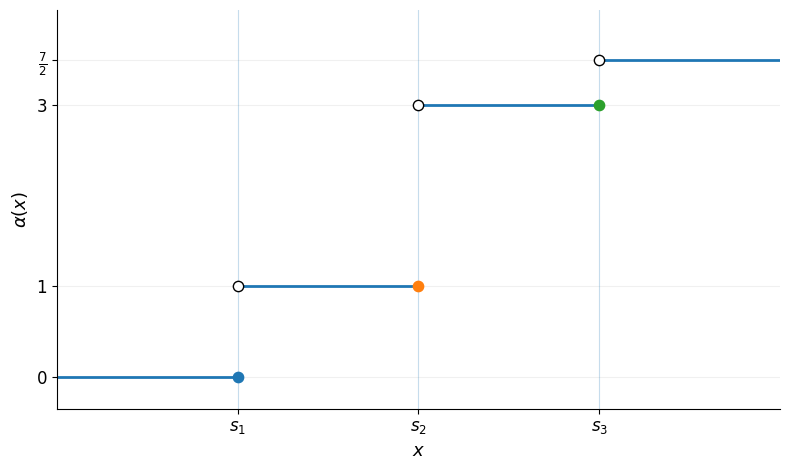
\includegraphics[width=0.5\textwidth]{
        CH6/images/Graph of a(x).png
    }
    \end{center}
\end{example}

\begin{theorem} \leavevmode \\
    \label{Thm6.15}
    Suppose $f: [a,b] \to \R$ is bounded, $s \in (a,b),$ $f$ is right continuous at $s$, and $\alpha(x) = I(x-s)$. Then $f \in R_\alpha[a,b]$ and $\int_a^b fd\alpha = f(s).$
\end{theorem}

\begin{proof}
    In what follows, we will introduce a sequence of partitions $(P_n)$ in $\Pi [a,b]$ such that 
    $$\lim_{n\to \infty} \left[U(f, \alpha, P_n) - L(f, \alpha, P_n)\right] = 0 \text{ and } \lim_{n\to \infty}U(f, \alpha, P_n) = \lim_{n\to\infty} L(f, \alpha,P_n) = f(s).$$
    This, according to the sequential criterion of integrability, tells us that 
    $$f \in R_\alpha [a,b] \text{ and } \int_a^b fd\alpha = f(s).$$
    Let $N$ be large enough so that $s + \frac{1}{N} < b.$ For each $n \geq N,$ let 
    $$P_n = \set{a, s, s+\frac{1}{n}, b}.$$
    We have 
    $$U(f, \alpha, P_n) = \sum_{k=1}^{3}M_k \Delta \alpha_k = M_2 \Delta \alpha_2 = \left[\sup_{s \leq x \leq s+ \frac{1}{n}}f(x)\right](1) = \sup_{s \leq x \leq s + \frac{1}{n}}f(x)$$
    $$L(f, \alpha, P_n) = \sum_{k=1}^{3}m_k \Delta \alpha_k = m_2 \Delta \alpha_2 = \left[\inf_{s \leq x \leq s+\frac{1}{n}}f(x)\right](1) = \inf_{s\leq x \leq s+ \frac{1}{n}}f(x).$$
    Therefore,
    $$\lim_{n\to \infty}U(f, \alpha, P_n) = \lim_{n\to \infty} \sup_{s \leq x \leq s + \frac{1}{n}}f(x) = f(x)$$
    $$\lim_{n \to \infty} L(f, \alpha, P_n) = \lim_{n \to \infty}\inf_{s \leq x \leq s+\frac{1}{n}}f(x) = f(x).$$
    Here, we are using the fact that $f$ is continuous at $s$, but right continuity would have been enough. We conclude that $\lim_{n \to \infty}\left[U(f, \alpha, P_n)- L(f, \alpha, P_n)\right] = f(s) - f(s) = 0,$ so $f \in R_\alpha[a,b]$ and $\int_a^bf d\alpha = \lim U(f, \alpha, P_n) = f(s).$
    \qed
\end{proof}

\begin{theorem} \leavevmode \\
    \label{Thm6.16}
    Suppose $\forall n \geq 1, c_n \geq 0,$ $\sum_{n=1}^{\infty}c_n$ converges. Let $s_1 < s_2< ... $ be points in $(a,b), \alpha:[a,b] \to \R, \alpha(x) = \sum_{n=1}^{\infty} c_n I(x-s_n),$ and $f:[a,b] \to \R$ be continuous. Then
    $$f\in R_\alpha[a,b] \text{ and } \int_a^bf d \alpha = \sum_{n=1}^{\infty}c_nf(s_n).$$
\end{theorem}
\newpage

\end{document}